\documentclass[conference]{IEEEtran}
% Target: arXiv cs.LG preprint only (RESEARCH-PLAN §1.2). IEEEtran two-column kept, <= 12 pages (§6 decision 8).
\usepackage[utf8]{inputenc}
\usepackage[T1]{fontenc}
\usepackage{amsmath,amssymb}
\usepackage{graphicx}
\usepackage{booktabs}
\usepackage{multirow}
\usepackage{xcolor}
\usepackage{url}
\usepackage[hidelinks]{hyperref}

\newcommand{\BSS}{\mathrm{BSS}}
\newcommand{\E}{\mathbb{E}}
% S1-2 learning curve (ml/forecast/out/learning_curve/summary.json)
\newcommand{\lcBestBssSeventyTwo}{0.83}
\newcommand{\lcTwelveKBssSeventyTwo}{0.67}
\newcommand{\lcBestStep}{88{,}000}
% S1-9 sample-count study (tab:samples)
% BEGIN samples (generated by ml/forecast/windows/samples.py tables from ml/forecast/out/samples/*.json; do not edit)
\newcommand{\llNFifty}{0.862}
\newcommand{\llNFiftyCI}{[0.81, 0.91]}
\newcommand{\bssNFifty}{0.849}
\newcommand{\bssNFiftyCI}{[0.83, 0.87]}
\newcommand{\bssDbNFifty}{0.852}
\newcommand{\floorPctNFifty}{1.55}
\newcommand{\llFloorNFifty}{0.143}
\newcommand{\llPredNFifty}{0.864}
\newcommand{\dllNFifty}{0.074}
\newcommand{\dllNFiftyCI}{[0.058, 0.091]}
\newcommand{\llNTwoHundred}{0.800}
\newcommand{\llNTwoHundredCI}{[0.76, 0.84]}
\newcommand{\bssNTwoHundred}{0.850}
\newcommand{\bssNTwoHundredCI}{[0.83, 0.87]}
\newcommand{\bssDbNTwoHundred}{0.851}
\newcommand{\floorPctNTwoHundred}{0.50}
\newcommand{\llFloorNTwoHundred}{0.046}
\newcommand{\llPredNTwoHundred}{0.805}
\newcommand{\dllNTwoHundred}{0.012}
\newcommand{\dllNTwoHundredCI}{[0.007, 0.017]}
\newcommand{\llNFiveHundred}{0.788}
\newcommand{\llNFiveHundredCI}{[0.75, 0.82]}
\newcommand{\bssNFiveHundred}{0.850}
\newcommand{\bssNFiveHundredCI}{[0.83, 0.87]}
\newcommand{\bssDbNFiveHundred}{0.850}
\newcommand{\floorPctNFiveHundred}{0.24}
\newcommand{\llFloorNFiveHundred}{0.022}
\newcommand{\llPredNFiveHundred}{0.794}
\newcommand{\floorHitsNFiveHundred}{16}
\newcommand{\nForecastsSamples}{6{,}780}
\newcommand{\nSeedsSamples}{60}
% END samples
% S1-5 200-seed evaluation (tab:bss, tab:scores, RQ1 text); v3 = median over three training seeds
% BEGIN e200 (generated by ml/forecast/figures_paper.py tables200 from ml/forecast/out/eval200/*.json; do not edit)
\newcommand{\bssGruSeventyTwo}{0.84}
\newcommand{\bssGruOneSixtyEight}{0.54}
\newcommand{\bssDiffTwoSeventyTwo}{0.83}
\newcommand{\bssDiffTwoOneSixtyEight}{0.55}
\newcommand{\bssDiffThreeSeventyTwo}{0.85}
\newcommand{\bssDiffThreeOneSixtyEight}{0.58}
\newcommand{\llDiffThree}{0.79}
\newcommand{\esDiffThree}{1.26}
\newcommand{\vsDiffThree}{16.9}
\newcommand{\bssPfSeventyTwo}{0.93}
\newcommand{\bssPfOneSixtyEight}{0.76}
\newcommand{\esGruPaths}{1.78}
\newcommand{\vsGruPaths}{22.2}
\newcommand{\bssClockSeventyTwo}{0.16}
\newcommand{\bssClockOneSixtyEight}{0.15}
\newcommand{\bssBotSeventyTwo}{0.17}
\newcommand{\bssBotOneSixtyEight}{0.15}
\newcommand{\bssDiffThreeSeventyTwoRange}{(0.846--0.849)}
\newcommand{\bssDiffThreeOneSixtyEightRange}{(0.575--0.578)}
\newcommand{\bssBotOverClockMax}{0.05}
\newcommand{\bssClockPfSeventyTwo}{0.92}
\newcommand{\bssClockPfOneSixtyEight}{0.72}
\newcommand{\bssClockGruSeventyTwo}{0.81}
\newcommand{\bssClockGruOneSixtyEight}{0.46}
\newcommand{\bssClockDiffTwoSeventyTwo}{0.80}
\newcommand{\bssClockDiffTwoOneSixtyEight}{0.47}
\newcommand{\bssClockDiffThreeSeventyTwo}{0.82}
\newcommand{\bssClockDiffThreeOneSixtyEight}{0.50}
\newcommand{\bssRowClock}{0.06 & 0.08 & 0.12 & 0.16 [0.15, 0.17] & 0.18 & 0.18 & 0.16 & 0.15 [0.13, 0.16]}
\newcommand{\bssRowBot}{0.10 & 0.10 & 0.13 & 0.17 [0.16, 0.18] & 0.19 & 0.19 & 0.17 & 0.15 [0.13, 0.16]}
\newcommand{\bssRowGru}{0.93 & 0.92 & 0.87 & 0.84 [0.83, 0.85] & 0.79 & 0.73 & 0.64 & 0.54 [0.53, 0.55]}
\newcommand{\bssRowDiffTwo}{0.93 & 0.92 & 0.87 & 0.83 [0.82, 0.85] & 0.79 & 0.72 & 0.64 & 0.55 [0.54, 0.56]}
\newcommand{\bssRowPf}{0.97 & 0.96 & 0.95 & 0.93 [0.93, 0.94] & 0.91 & 0.87 & 0.82 & 0.76 [0.75, 0.78]}
\newcommand{\bssRowDiffThree}{0.94 & 0.93 & 0.88 & 0.85 (0.846--0.849) & 0.81 & 0.75 & 0.67 & 0.58 (0.575--0.578)}
\newcommand{\scRowClim}{30.0 & 2.51 & 54.1 & 1.96 & 3.64 & 65.5}
\newcommand{\scRowClock}{25.2 & 2.23 & 44.4 & 1.69 & 3.25 & 56.3}
\newcommand{\scRowBot}{25.0 & 2.19 & 44.1 & 1.66 & -- & --}
\newcommand{\scRowGru}{7.7 & 0.85 & 11.5 & 0.43 & 1.78 & 22.2}
\newcommand{\scRowDiffTwo}{7.7 & 0.84 & 11.0 & 0.45 & 1.34 & 18.1}
\newcommand{\scRowDiffThree}{7.2 & 0.79 & 10.4 & 0.41 & 1.26 & 16.9}
\newcommand{\scRowPf}{3.6 & 0.52 & -- & -- & 0.87 & 9.6}
\newcommand{\esCiMax}{0.03}
\newcommand{\vsCiMax}{0.8}
\newcommand{\crpsGru}{7.7}
\newcommand{\crpsDiffTwo}{7.7}
\newcommand{\crpsPf}{3.6}
\newcommand{\crpsDiffThree}{7.2}
\newcommand{\crpsDiffThreeRange}{(7.1--7.2)}
\newcommand{\wGru}{11.5}
\newcommand{\wDiffTwo}{11.0}
\newcommand{\wDiffThree}{10.4}
\newcommand{\llGru}{0.85}
\newcommand{\llDiffTwo}{0.84}
\newcommand{\esDiffTwo}{1.34}
\newcommand{\vsDiffTwo}{18.1}
\newcommand{\esDiffThreeRange}{(1.26--1.27)}
\newcommand{\vsDiffThreeRange}{(16.8--16.9)}
\newcommand{\esPf}{0.87}
\newcommand{\vsPf}{9.6}
\newcommand{\esClimPaths}{3.64}
\newcommand{\vsClimPaths}{65.5}
\newcommand{\esClockPaths}{3.25}
\newcommand{\vsClockPaths}{56.3}
\newcommand{\pbFallback}{9{,}046}
\newcommand{\pbDraws}{4{,}520{,}000}
\newcommand{\pathsDiff}{200}
\newcommand{\ddimSteps}{50}
\newcommand{\pathsAnalogue}{200}
\newcommand{\gpuHoursTwo}{1.3}
\newcommand{\gpuHoursThreeMin}{12.7}
\newcommand{\gpuHoursThreeMax}{14.9}
\newcommand{\exLandHours}{68}
\newcommand{\exIssueDay}{10}
\newcommand{\exSeed}{220000}
\newcommand{\exPeakDiff}{0.99}
\newcommand{\exPeakPf}{1.00}
% END e200
% S1-12 wind-noise ablation (tab:windnoise, Limitations); 60 test seeds, original murky = same models on the same seeds
% BEGIN wn (generated by ml/forecast/windows/windnoise.py tex from ml/forecast/out/windnoise/{summary_endurance_murky_windnoise,ref60/summary_endurance_murky,done,diff,gru,pf}.json; do not edit)
\newcommand{\wnPfBssSeventyTwo}{0.91}
\newcommand{\wnRefPfBssSeventyTwo}{0.94}
\newcommand{\wnPfBssOneSixtyEight}{0.68}
\newcommand{\wnRefPfBssOneSixtyEight}{0.78}
\newcommand{\wnRowPf}{0.94 [0.93, 0.95] & 0.91 [0.90, 0.92] & 0.78 [0.76, 0.80] & 0.68 [0.66, 0.71]}
\newcommand{\wnGruBssSeventyTwo}{0.81}
\newcommand{\wnRefGruBssSeventyTwo}{0.83}
\newcommand{\wnGruBssOneSixtyEight}{0.50}
\newcommand{\wnRefGruBssOneSixtyEight}{0.53}
\newcommand{\wnRowGru}{0.83 [0.81, 0.85] & 0.81 [0.79, 0.84] & 0.53 [0.50, 0.56] & 0.50 [0.47, 0.53]}
\newcommand{\wnDiffBssSeventyTwo}{0.82}
\newcommand{\wnRefDiffBssSeventyTwo}{0.85}
\newcommand{\wnDiffBssOneSixtyEight}{0.52}
\newcommand{\wnRefDiffBssOneSixtyEight}{0.57}
\newcommand{\wnRowDiff}{0.85 [0.83, 0.87] & 0.82 [0.80, 0.84] & 0.57 [0.54, 0.60] & 0.52 [0.49, 0.55]}
\newcommand{\wnSeeds}{60}
\newcommand{\wnPaths}{200}
\newcommand{\wnDdim}{50}
\newcommand{\wnDiffSteps}{100{,}000}
\newcommand{\wnGpuHours}{8.8}
\newcommand{\wnCpuHours}{4.6}
% END wn
% S1-11c rungs 3a' (daily GRU table) and 3b (daily diffusion table): tab:storms / tab:ladder rows and RQ2 text
% BEGIN e0b (generated by ml/forecast/figures_paper.py storms3b from ml/forecast/out/storm_seeds_*.json; do not edit)
\newcommand{\ebFcdDeathsG}{1.77}
\newcommand{\ebFcdDeathsGMin}{0.87}
\newcommand{\ebFcdDeathsGMax}{2.28}
\newcommand{\ebFcdDeathsGRuns}{2.28, 2.15, 0.87}
\newcommand{\ebFcdDaysG}{54.4}
\newcommand{\ebFcdDaysGMin}{45.7}
\newcommand{\ebFcdDaysGMax}{65.3}
\newcommand{\ebFcdDaysGRuns}{45.7, 52.2, 65.3}
\newcommand{\ebFcdStormsG}{3.9}
\newcommand{\ebFcdStormsGMin}{3.2}
\newcommand{\ebFcdStormsGMax}{4.8}
\newcommand{\ebFcdStormsGRuns}{3.2, 3.7, 4.8}
\newcommand{\ebFcdCapG}{10}
\newcommand{\ebFcdCapGMin}{0}
\newcommand{\ebFcdCapGMax}{28}
\newcommand{\ebFcdCapGRuns}{0, 1, 28}
\newcommand{\ebFcdExiledG}{57}
\newcommand{\ebFcdExiledGMin}{32}
\newcommand{\ebFcdExiledGMax}{77}
\newcommand{\ebFcdExiledGRuns}{77, 62, 32}
\newcommand{\ebFcdAnyG}{34}
\newcommand{\ebFcgDeathsG}{1.92}
\newcommand{\ebFcgDeathsGMin}{1.83}
\newcommand{\ebFcgDeathsGMax}{1.99}
\newcommand{\ebFcgDeathsGRuns}{1.83, 1.92, 1.99}
\newcommand{\ebFcgDaysG}{59.1}
\newcommand{\ebFcgDaysGMin}{56.1}
\newcommand{\ebFcgDaysGMax}{62.7}
\newcommand{\ebFcgDaysGRuns}{62.7, 58.7, 56.1}
\newcommand{\ebFcgStormsG}{4.3}
\newcommand{\ebFcgStormsGMin}{4.1}
\newcommand{\ebFcgStormsGMax}{4.6}
\newcommand{\ebFcgStormsGRuns}{4.6, 4.2, 4.1}
\newcommand{\ebFcgCapG}{2}
\newcommand{\ebFcgCapGMin}{1}
\newcommand{\ebFcgCapGMax}{4}
\newcommand{\ebFcgCapGRuns}{4, 1, 2}
\newcommand{\ebFcgExiledG}{53}
\newcommand{\ebFcgExiledGMin}{40}
\newcommand{\ebFcgExiledGMax}{74}
\newcommand{\ebFcgExiledGRuns}{46, 74, 40}
\newcommand{\ebFcgAnyG}{34}
\newcommand{\ebFcdFcgDeathsG}{$+$0.22}
\newcommand{\ebFcdFcgDeathsGCI}{[0.11, 0.32]}
\newcommand{\ebFcdFcgDeathsGRuns}{$+$0.97, $+$0.45, $-$0.76}
\newcommand{\ebFcdFcgDeathsGBelow}{1}
\newcommand{\ebFcdFcgDeathsGAbove}{2}
\newcommand{\ebFcdFcgAnyG}{$+$4.3}
\newcommand{\ebFcdFcgAnyGCI}{[2.8, 5.8]}
\newcommand{\ebFcdFcgAnyGRuns}{$+$16.7, $+$7.8, $-$11.7}
\newcommand{\ebFcdFcgAnyGBelow}{1}
\newcommand{\ebFcdFcgAnyGAbove}{2}
\newcommand{\ebFcdFcgRateG}{$+$1.0}
\newcommand{\ebFcdFcgRateGCI}{[0.5, 1.5]}
\newcommand{\ebFcdFcgRateGRuns}{$+$4.0, $+$2.6, $-$3.6}
\newcommand{\ebFcdFcgRateGBelow}{1}
\newcommand{\ebFcdFcgRateGAbove}{2}
\newcommand{\ebFcdFcgDaysG}{$-$4.7}
\newcommand{\ebFcdFcgDaysGCI}{[$-$5.9, $-$3.6]}
\newcommand{\ebFcdFcgDaysGRuns}{$-$16.9, $-$6.5, $+$9.3}
\newcommand{\ebFcdFcgDaysGBelow}{2}
\newcommand{\ebFcdFcgDaysGAbove}{1}
\newcommand{\ebFcdFcDeathsG}{$+$0.24}
\newcommand{\ebFcdFcDeathsGCI}{[0.14, 0.34]}
\newcommand{\ebFcdFcDeathsGRuns}{$+$0.29, $+$1.16, $-$0.73}
\newcommand{\ebFcdFcDeathsGBelow}{1}
\newcommand{\ebFcdFcDeathsGAbove}{2}
\newcommand{\ebFcdFcAnyG}{$+$4.9}
\newcommand{\ebFcdFcAnyGCI}{[3.4, 6.3]}
\newcommand{\ebFcdFcAnyGRuns}{$+$6.3, $+$13.6, $-$5.3}
\newcommand{\ebFcdFcAnyGBelow}{1}
\newcommand{\ebFcdFcAnyGAbove}{2}
\newcommand{\ebFcdFcRateG}{$+$1.3}
\newcommand{\ebFcdFcRateGCI}{[0.8, 1.7]}
\newcommand{\ebFcdFcRateGRuns}{$+$1.0, $+$4.7, $-$1.9}
\newcommand{\ebFcdFcRateGBelow}{1}
\newcommand{\ebFcdFcRateGAbove}{2}
\newcommand{\ebFcdFcDaysG}{$-$7.2}
\newcommand{\ebFcdFcDaysGCI}{[$-$8.3, $-$6.0]}
\newcommand{\ebFcdFcDaysGRuns}{$+$0.9, $-$32.0, $+$9.5}
\newcommand{\ebFcdFcDaysGBelow}{1}
\newcommand{\ebFcdFcDaysGAbove}{1}
\newcommand{\ebFcdDeathsS}{1.47}
\newcommand{\ebFcdDeathsSMin}{0.79}
\newcommand{\ebFcdDeathsSMax}{1.89}
\newcommand{\ebFcdDeathsSRuns}{1.72, 1.89, 0.79}
\newcommand{\ebFcdDaysS}{55.8}
\newcommand{\ebFcdDaysSMin}{49.3}
\newcommand{\ebFcdDaysSMax}{66.6}
\newcommand{\ebFcdDaysSRuns}{49.3, 51.5, 66.6}
\newcommand{\ebFcdStormsS}{4.0}
\newcommand{\ebFcdStormsSMin}{3.5}
\newcommand{\ebFcdStormsSMax}{4.9}
\newcommand{\ebFcdStormsSRuns}{3.5, 3.6, 4.9}
\newcommand{\ebFcdCapS}{10}
\newcommand{\ebFcdCapSMin}{0}
\newcommand{\ebFcdCapSMax}{31}
\newcommand{\ebFcdCapSRuns}{0, 0, 31}
\newcommand{\ebFcdExiledS}{76}
\newcommand{\ebFcdExiledSMin}{48}
\newcommand{\ebFcdExiledSMax}{92}
\newcommand{\ebFcdExiledSRuns}{92, 87, 48}
\newcommand{\ebFcdAnyS}{27}
\newcommand{\ebFcgDeathsS}{1.53}
\newcommand{\ebFcgDeathsSMin}{1.49}
\newcommand{\ebFcgDeathsSMax}{1.55}
\newcommand{\ebFcgDeathsSRuns}{1.55, 1.49, 1.53}
\newcommand{\ebFcgDaysS}{54.4}
\newcommand{\ebFcgDaysSMin}{53.8}
\newcommand{\ebFcgDaysSMax}{54.9}
\newcommand{\ebFcgDaysSRuns}{54.6, 54.9, 53.8}
\newcommand{\ebFcgStormsS}{3.9}
\newcommand{\ebFcgStormsSMin}{3.9}
\newcommand{\ebFcgStormsSMax}{3.9}
\newcommand{\ebFcgStormsSRuns}{3.9, 3.9, 3.9}
\newcommand{\ebFcgCapS}{1}
\newcommand{\ebFcgCapSMin}{0}
\newcommand{\ebFcgCapSMax}{1}
\newcommand{\ebFcgCapSRuns}{1, 0, 1}
\newcommand{\ebFcgExiledS}{86}
\newcommand{\ebFcgExiledSMin}{85}
\newcommand{\ebFcgExiledSMax}{88}
\newcommand{\ebFcgExiledSRuns}{88, 86, 85}
\newcommand{\ebFcgAnyS}{29}
\newcommand{\ebFcdFcgDeathsS}{$+$0.14}
\newcommand{\ebFcdFcgDeathsSCI}{[0.06, 0.23]}
\newcommand{\ebFcdFcgDeathsSRuns}{$+$0.33, $+$0.51, $-$0.41}
\newcommand{\ebFcdFcgDeathsSBelow}{1}
\newcommand{\ebFcdFcgDeathsSAbove}{2}
\newcommand{\ebFcdFcgAnyS}{$+$0.8}
\newcommand{\ebFcdFcgAnySCI}{[$-$0.4, 2.0]}
\newcommand{\ebFcdFcgAnySRuns}{$+$2.4, $+$6.8, $-$6.8}
\newcommand{\ebFcdFcgAnySBelow}{1}
\newcommand{\ebFcdFcgAnySAbove}{2}
\newcommand{\ebFcdFcgRateS}{$+$0.8}
\newcommand{\ebFcdFcgRateSCI}{[0.5, 1.1]}
\newcommand{\ebFcdFcgRateSRuns}{$+$0.8, $+$1.9, $-$0.4}
\newcommand{\ebFcdFcgRateSBelow}{0}
\newcommand{\ebFcdFcgRateSAbove}{2}
\newcommand{\ebFcdFcgDaysS}{$+$1.4}
\newcommand{\ebFcdFcgDaysSCI}{[0.3, 2.5]}
\newcommand{\ebFcdFcgDaysSRuns}{$-$5.3, $-$3.4, $+$12.8}
\newcommand{\ebFcdFcgDaysSBelow}{2}
\newcommand{\ebFcdFcgDaysSAbove}{1}
\newcommand{\ebFcdFcDeathsS}{$+$0.07}
\newcommand{\ebFcdFcDeathsSCI}{[$-$0.02, 0.16]}
\newcommand{\ebFcdFcDeathsSRuns}{$-$0.51, $+$1.11, $-$0.39}
\newcommand{\ebFcdFcDeathsSBelow}{2}
\newcommand{\ebFcdFcDeathsSAbove}{1}
\newcommand{\ebFcdFcAnyS}{$+$0.4}
\newcommand{\ebFcdFcAnySCI}{[$-$0.8, 1.6]}
\newcommand{\ebFcdFcAnySRuns}{$-$8.1, $+$12.3, $-$3.0}
\newcommand{\ebFcdFcAnySBelow}{2}
\newcommand{\ebFcdFcAnySAbove}{1}
\newcommand{\ebFcdFcRateS}{$-$0.2}
\newcommand{\ebFcdFcRateSCI}{[$-$0.5, 0.2]}
\newcommand{\ebFcdFcRateSRuns}{$-$2.7, $+$3.0, $-$0.9}
\newcommand{\ebFcdFcRateSBelow}{2}
\newcommand{\ebFcdFcRateSAbove}{1}
\newcommand{\ebFcdFcDaysS}{$-$1.9}
\newcommand{\ebFcdFcDaysSCI}{[$-$3.1, $-$0.7]}
\newcommand{\ebFcdFcDaysSRuns}{$+$8.3, $-$33.2, $+$19.2}
\newcommand{\ebFcdFcDaysSBelow}{1}
\newcommand{\ebFcdFcDaysSAbove}{2}
\newcommand{\ebCapMaxRunOne}{4}
\newcommand{\ebIssueHour}{07:00}
\newcommand{\ebTableDdim}{25}
\newcommand{\ebTablePaths}{50}
\newcommand{\ebTableSeeds}{1{,}000}
\newcommand{\ebTableDiffHours}{16.6}
\newcommand{\ebTableGruMin}{3}
\newcommand{\ebPpoHoursMin}{53}
\newcommand{\ebPpoHoursMax}{57}
\newcommand{\ebStepsPerRound}{42{,}082}
% END e0b
% BEGIN e18 (generated by ml/forecast/windows/secondary.py tex from ml/forecast/out/eval200/summary_{endurance_clear,a_new_home_murky}.json; do not edit)
\newcommand{\secClearClockSeventyTwo}{0.16}
\newcommand{\secClearClockOneSixtyEight}{0.15}
\newcommand{\secClearClockCrps}{25.23}
\newcommand{\secClearGruSeventyTwo}{0.91}
\newcommand{\secClearGruOneSixtyEight}{0.68}
\newcommand{\secClearGruCrps}{4.67}
\newcommand{\secClearDiffSeventyTwo}{0.93}
\newcommand{\secClearDiffOneSixtyEight}{0.76}
\newcommand{\secClearDiffCrps}{3.79}
\newcommand{\secClearPfSeventyTwo}{0.96}
\newcommand{\secClearPfOneSixtyEight}{0.86}
\newcommand{\secClearPfCrps}{2.08}
\newcommand{\secClearDiffEs}{0.71}
\newcommand{\secClearPfEs}{0.53}
\newcommand{\secHomeClockSeventyTwo}{0.26}
\newcommand{\secHomeClockOneSixtyEight}{0.39}
\newcommand{\secHomeClockCrps}{17.83}
\newcommand{\secHomeGruSeventyTwo}{0.84}
\newcommand{\secHomeGruOneSixtyEight}{0.66}
\newcommand{\secHomeGruCrps}{5.84}
\newcommand{\secHomeDiffSeventyTwo}{0.85}
\newcommand{\secHomeDiffOneSixtyEight}{0.70}
\newcommand{\secHomeDiffCrps}{5.22}
\newcommand{\secHomePfSeventyTwo}{0.95}
\newcommand{\secHomePfOneSixtyEight}{0.86}
\newcommand{\secHomePfCrps}{2.12}
\newcommand{\secHomeDiffEs}{1.14}
\newcommand{\secHomePfEs}{0.72}
% END e18

% BEGIN review (generated by docs/paper/review_macros.py from ml/forecast/out/{value_curve,marginal/{paired,summary_endurance_murky},learning_curve/summary}.json; do not edit)
\newcommand{\vcClockSeventyTwo}{0.37}
\newcommand{\vcClockOneSixtyEight}{0.03}
\newcommand{\vcClockPeak}{0.44}
\newcommand{\vcBotSeventyTwo}{0.38}
\newcommand{\vcBotOneSixtyEight}{0.03}
\newcommand{\vcBotPeak}{0.46}
\newcommand{\vcGruSeventyTwo}{0.88}
\newcommand{\vcGruSeventyTwoCI}{[0.87, 0.89]}
\newcommand{\vcGruOneSixtyEight}{0.36}
\newcommand{\vcGruPeak}{0.91}
\newcommand{\vcDiffTwoSeventyTwo}{0.89}
\newcommand{\vcDiffTwoSeventyTwoCI}{[0.88, 0.90]}
\newcommand{\vcDiffTwoOneSixtyEight}{0.42}
\newcommand{\vcDiffTwoPeak}{0.91}
\newcommand{\vcPfSeventyTwo}{0.94}
\newcommand{\vcPfSeventyTwoCI}{[0.93, 0.95]}
\newcommand{\vcPfOneSixtyEight}{0.56}
\newcommand{\vcPfPeak}{0.96}
\newcommand{\vcDiffThreeSeventyTwo}{0.89}
\newcommand{\vcDiffThreeSeventyTwoRange}{0.89--0.90}
\newcommand{\vcDiffThreeOneSixtyEight}{0.44}
\newcommand{\vcDiffThreePeak}{0.92}
\newcommand{\vcBaseRateSeventyTwo}{0.23}
\newcommand{\mcBssSeventyTwo}{$+$0.016}
\newcommand{\mcBssSeventyTwoCI}{[0.006, 0.025]}
\newcommand{\mcBssOneSixtyEight}{$+$0.035}
\newcommand{\mcBssOneSixtyEightCI}{[0.021, 0.049]}
\newcommand{\mcEs}{$+$0.21}
\newcommand{\mcEsCI}{[0.19, 0.23]}
\newcommand{\mcVs}{$-$0.64}
\newcommand{\mcVsCI}{[$-$1.05, $-$0.24]}
\newcommand{\mcEsShuf}{$+$0.32}
\newcommand{\mcEsShufCI}{[0.30, 0.33]}
\newcommand{\mcVsShuf}{$+$1.11}
\newcommand{\mcVsShufCI}{[0.91, 1.32]}
\newcommand{\mcEsMargShuf}{$-$0.11}
\newcommand{\mcEsMargShufCI}{[$-$0.12, $-$0.09]}
\newcommand{\mcVsMargShuf}{$-$1.75}
\newcommand{\mcVsMargShufCI}{[$-$2.10, $-$1.41]}
\newcommand{\mcRowJoint}{0.84 [0.82, 0.86] & 0.56 [0.53, 0.58] & 1.30 [1.26, 1.34] & 17.4 [16.5, 18.2]}
\newcommand{\mcRowMarg}{0.86 [0.84, 0.88] & 0.59 [0.56, 0.62] & 1.51 [1.46, 1.56] & 16.7 [15.8, 17.6]}
\newcommand{\mcRowShuf}{-- & -- & 1.61 [1.57, 1.66] & 18.5 [17.6, 19.4]}
\newcommand{\mcEsRelPct}{16}
\newcommand{\lcBestBssSeventyTwoCI}{[0.82, 0.85]}
\newcommand{\lcBestBssOneSixtyEight}{0.54}
\newcommand{\lcTwelveKBssSeventyTwoCI}{[0.65, 0.69]}
\newcommand{\lcTwelveKBssOneSixtyEight}{0.33}
\newcommand{\lcBestValLoss}{0.165}
\newcommand{\lcTwelveKValLoss}{0.211}
% END review

\begin{document}

\title{Imagining Winter: Generative Storm Forecasts and the Value of Foresight in a Chaotic Survival Game}

\author{\IEEEauthorblockN{Zhenzhou (Luke) Shi}
\IEEEauthorblockA{Independent Researcher\\
Email: \href{mailto:szz185@gmail.com}{szz185@gmail.com}}}

\maketitle

\begin{abstract}
Survival games ask players to prepare days ahead for weather they can only
infer from ambiguous signs. We build a controlled testbed from \emph{Last
Embers}, a bit-exact survival simulation whose blizzards come from an
integer fixed-point Lorenz-63 system and are observed only through noisy
precursors. Because the generator is known exactly, a particle filter on the
game's own dynamics gives a near-exact predictive distribution (PIT deciles
$0.094$--$0.107$ over $22{,}600$ forecasts) against which learned forecasters
are graded. \textbf{RQ1:} over 200 test seeds, a conditional diffusion model
that generates seven-day weather trajectories (transformer denoiser, median of
three training seeds) reaches a 72-hour Brier skill of
$\bssDiffThreeSeventyTwo$, a U-Net diffusion model $\bssDiffTwoSeventyTwo$, a
GRU that predicts the landing time directly $\bssGruSeventyTwo$, a
time-since-last-storm clock $\bssClockSeventyTwo$ and the filter
$\bssPfSeventyTwo$; on the trajectories the transformer model's energy score
is $\esDiffThree$, against $\esGruPaths$ for real analogues stitched behind
the GRU forecast and $\esPf$ for the filter. \textbf{RQ2:} in a
value-of-information ladder of PPO colony managers (no signs, raw signs,
signs plus a forecast, oracle storm date; three training runs each), most
episodes end in exile or a furnace explosion rather than in storm deaths, so
we measure losses per storm reached. The oracle date lowers deaths per storm
relative to raw signs in every run ($-0.78$ [$-0.88$, $-0.66$], greedy);
raw signs give no reliable benefit, the folk omens of the studied snapshot
carry no lead time, and a linear probe finds no implicit forecast in the
sign-reading agent. The GRU forecast as an extra input lowers deaths per
storm relative to raw signs in every run ($-1.26$ [$-1.38$, $-1.15$]).
Matched once-daily forecasts from the diffusion model and the GRU differ by
\ebFcdFcgDeathsG{} deaths per storm \ebFcdFcgDeathsGCI{}, with training runs
of both signs, so three runs cannot order the two forecasters as policy
inputs.
\end{abstract}

\begin{IEEEkeywords}
probabilistic forecasting, diffusion models, value of information,
reinforcement learning, survival games, chaotic dynamics
\end{IEEEkeywords}

%======================================================================
\section{Introduction}
%======================================================================
Colony-survival games such as \emph{Frostpunk}~\cite{frostpunk2018} build their
tension around a known, approaching hazard: a great storm that will kill the
unprepared. In most commercial games the hazard is scripted, so
that ``forecasting'' collapses into memorising a calendar. When the hazard is
instead driven by a chaotic process and revealed only through noisy signs, the
game poses a genuine sequential inference problem: a good player must integrate
days of ambiguous evidence into a belief about \emph{when} the storm will land,
and then decide how much coal, food and shelter to commit before it does.

This setting is attractive for game-AI research for three reasons. First, the
weather is \emph{exogenous}~\cite{dietterich2018,sinclair2022}: nothing the
colony does changes it, so forecasting can be studied separately from control
and then reconnected through the value of the forecast. Second, when the weather
generator is known exactly, the true predictive distribution
$p(\text{future}\mid\text{signs so far})$ can be approximated to high
accuracy by sequential Monte Carlo~\cite{gordon1993,doucet2011}, giving every
learned forecaster an absolute yardstick that real-world weather never
provides. Third, chaos supplies a natural, smoothly decaying predictability
horizon~\cite{lorenz1963,sprott2003}, so forecast skill varies across exactly
the lead times (one to seven days) over which preparation decisions are made.

Generative models, and diffusion models in particular, are now the state of the
art in probabilistic medium-range weather forecasting~\cite{price2025gencast} and are used
increasingly to produce scenarios for downstream
decision-making~\cite{zarifis2025mpc,zarifis2025tree}. A diffusion forecaster
samples entire trajectories, so in principle it captures the joint temporal
structure that a planner needs (``the pressure drops for two days, \emph{then}
the storm lands'') rather than a separate marginal per lead time. Whether this
is an advantage when the question is simply ``when does the storm land?'' is
an empirical matter, which we measure against a direct landing-time classifier
and against the oracle.

\paragraph*{Contributions}
\begin{enumerate}
\item \textbf{A testbed with a verified oracle.} A bit-exact survival
simulation whose storms emerge from integer Lorenz-63 dynamics and are seen
only through noisy precursors, with leakage audit, disjoint seed splits and a
particle filter on the exact dynamics whose convergence and calibration we
check (Sections~\ref{sec:testbed}--\ref{sec:oracle}).
\item \textbf{RQ1: a forecasting comparison against the oracle.} Climatology,
a clock hazard, the game's warning rule, a GRU landing-time classifier and
two conditional diffusion models (U-Net and transformer denoisers), scored
against the outcome and the oracle on events and seven-day trajectories
(Section~\ref{sec:rq1}).
\item \textbf{RQ2: the value of foresight.} A ladder of PPO
agents~\cite{schulman2017ppo} fine-tuned from one checkpoint with increasing
weather information, and a linear probe for an implicit forecast
(Section~\ref{sec:rq2}), evaluated per storm reached with three training runs
per rung, including rungs fed by a GRU forecast and by a matched once-daily
diffusion forecast.
\item \textbf{Release.} Code (simulator core and weather generator,
oracle, baselines, forecasters, evaluation and PPO scripts) at
\url{https://github.com/gentoo111/imagining-winter} under the MIT License;
forecasts, result files and checkpoints as release assets
(\url{https://github.com/gentoo111/imagining-winter/releases/tag/v1.0})
under CC BY 4.0.
\end{enumerate}

%======================================================================
\section{Related Work}\label{sec:related}
%======================================================================
\paragraph*{Probabilistic and generative forecasting}
Diffusion models for time series include autoregressive
(TimeGrad~\cite{rasul2021timegrad}) and non-autoregressive designs, trained
conditionally (CSDI~\cite{tashiro2021csdi}) or trained unconditionally and
conditioned at sampling time (TSDiff~\cite{kollovieh2023tsdiff},
Diffusion-TS~\cite{yuan2024diffusionts}); see~\cite{lin2023survey}.
GenCast~\cite{price2025gencast} established diffusion ensembles for
medium-range weather, and DYffusion~\cite{cachay2023dyffusion} couples
diffusion with dynamics. Score-based data assimilation~\cite{rozet2023sda}
compares diffusion posteriors with a large-particle reference posterior on
Lorenz-63, and recent work corrects guided diffusion surrogates with
particle-filter resampling on Lorenz-63~\cite{wei2026surge} or checks whether AI ensembles sample the
correct conditional distribution~\cite{howard2026ensembles}. For generators
that expose only samples, randomized PIT values can be recalibrated into a
full predictive distribution~\cite{wang2026calibrated}. Calibration of
learned world models against known distributions has been studied for video
models~\cite{sadeghi2026calibench}, and model-based RL world models have been
tested under controlled stochasticity~\cite{barsainyan2025stori}.
We do not claim novelty for calibrating a generator against a known simulator
posterior; our contribution is to measure that calibration in a game and to
connect it to decision value in the same environment.

\paragraph*{Chaos and extremes as benchmarks}
Chaotic systems are established forecasting benchmarks~\cite{gilpin2021},
and ChaosBench~\cite{nathaniel2024chaosbench} benchmarks data-driven
subseasonal-to-seasonal climate prediction, where the butterfly effect limits
predictability; predictability of extremes and their precursors is
studied in~\cite{sterk2012,farazmand2019,guth2019,katsidoniotaki2026}. RL has
been applied to data assimilation in Lorenz-63~\cite{hammoud2024}, to control
of partially observed chaotic flows~\cite{weissenbacher2025}, and MPC with
assimilation has been used to steer Lorenz-63 into a prescribed
regime~\cite{kawasaki2024}. Those works control or estimate the chaotic system;
our agents cannot influence the weather and must prepare for it.

\paragraph*{Value of forecasts for sequential decisions}
The cost--loss framework~\cite{richardson2000,zhu2002} and its critiques
\cite{millner2009} quantify forecast value for static decisions. In RL,
forecast visibility has been studied for reservoir
operation~\cite{zanutto2025}, heat pumps (where forecasts added little
value)~\cite{schmitz2024} and demand response~\cite{ruelens2015}, and RL has
been applied to crop management under weather
variability~\cite{gautron2022gymdssat,
overweg2021cropgym,turchetta2022cyclesgym,wang2024pomdpag}. In
battery-storage dispatch, the value of price forecasts tracks their rank
correlation more than their absolute error~\cite{falezza2026rank}. Diffusion
forecasts have been fed to MPC and compared with model-free RL in energy
arbitrage~\cite{zarifis2025mpc} and used for scenario
generation~\cite{zarifis2025tree,sun2026diff2sp,zhou2026dfsg}. None of these
offers an exact predictive reference, chaotic precursor-only observation, or a
game setting.

\paragraph*{Diffusion for decision-making and game AI}
Diffusion planners~\cite{janner2022diffuser,ajay2023decisiondiffuser,
zhou2024dmpc} and policies~\cite{ren2025dppo,ma2025discretediffusionrl} are
active areas; in this paper the diffusion model is used only as a forecaster.
Open-ended survival benchmarks such as Crafter~\cite{hafner2022crafter} and
Craftax~\cite{matthews2024craftax} have hazards such as night-time zombies,
but none whose arrival has to be forecast from precursor signs.
A systematic search in November 2026 (OpenAlex and web search over 2025--2026
work on diffusion forecasting with reference posteriors, value of forecasts
for RL, and survival and colony games) found no colony-survival game used as
an RL or forecasting testbed, and no study that grades learned forecasters
against an exact simulator posterior and measures the forecast's value to an
RL agent in the same environment.

%======================================================================
\section{Testbed}\label{sec:testbed}
%======================================================================
\subsection{Game}
\emph{Last Embers} is a single-player colony-survival game. The player (or
agent) manages a camp of named survivors around a central furnace: assigning
workers to gather coal, wood and food, building shelter and heaters, researching
technology, enacting laws and sending scouting parties, while the outdoor
temperature falls. Periodic multi-day storms bring extreme cold; a camp that
has not stockpiled fuel and shelter loses people. The RL interface exposes a
128-dimensional observation and 94 masked discrete actions per in-game hour;
the reward is survival time and the number of people alive, with no
hand-written shaping. We use the HARDCORE difficulty on the \emph{Endurance}
profile (open-ended survival) and also the \emph{A New Home} scenario profile
for forecasting. Fig.~\ref{fig:testbed} shows one 120-day weather trace.

\begin{figure*}[t]
\centering
\begin{minipage}[b]{0.40\textwidth}\centering

\includegraphics[width=\linewidth]{figures/testbed_storm.png}\\
{\small (a)}
\end{minipage}\hfill
\begin{minipage}[b]{0.58\textwidth}\centering
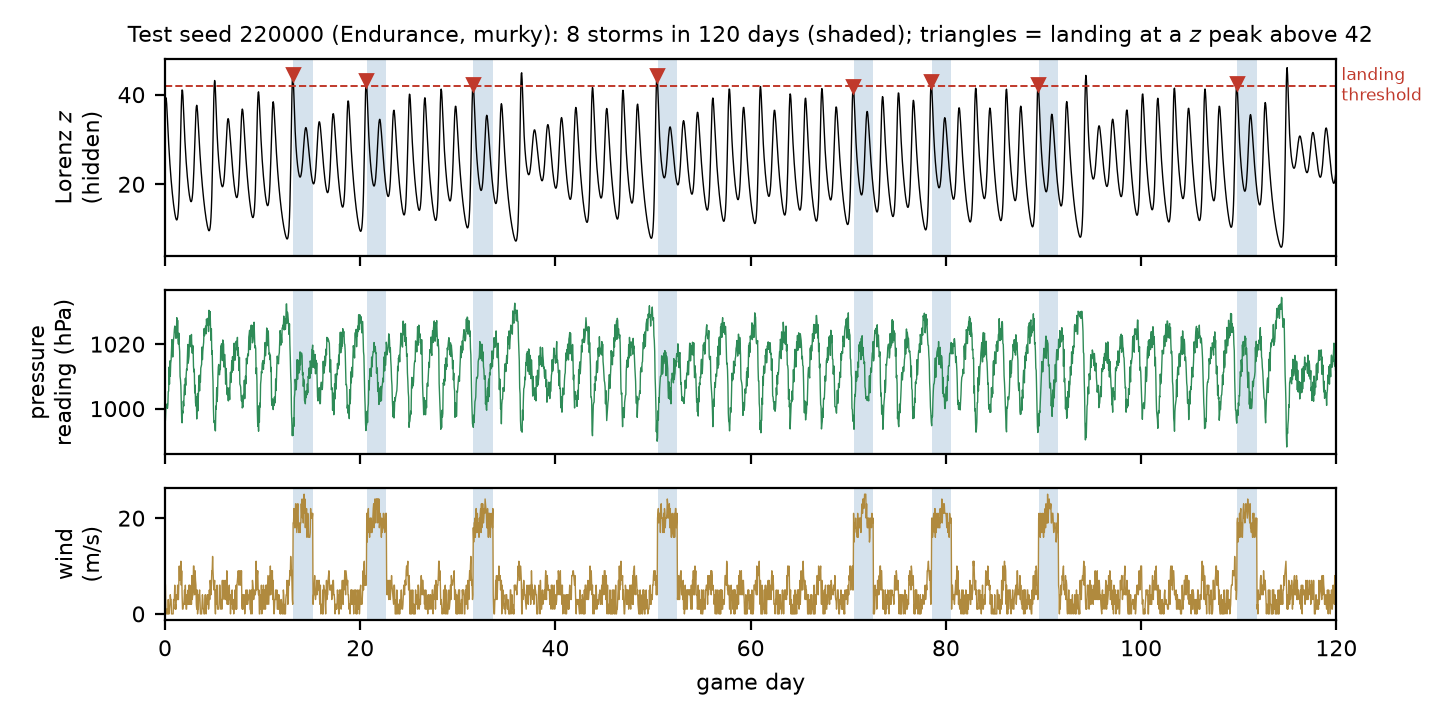
\includegraphics[width=\linewidth]{figures/testbed_trace.png}\\
{\small (b)}
\end{minipage}
\caption{The testbed. (a) The frozen build during a storm (A New Home,
chaotic weather, map seed 3, scripted bot; day 37, inside the great storm;
the interface is in Chinese): day and time, outdoor temperature
($-90\,^\circ$C), storm flag, furnace, population and stocks, pressure, trend,
wind and the daily animal and sky signs; event log top right. (b) Weather on
test seed 220000 (Endurance, murky): hidden Lorenz $z$ with storm landings
(triangles; a storm lands at an hourly $z$ peak above 42 once the day-8 and
four-day-gap conditions hold, and lasts two days, shaded), and the hourly
pressure and wind-speed readings the player sees.}
\label{fig:testbed}
\end{figure*}

\subsection{Chaotic weather}
The storm generator is the classic Lorenz-63 system~\cite{lorenz1963}
($\sigma{=}10$, $\rho{=}28$, $\beta{=}8/3$) integrated in Q16 fixed-point
integer arithmetic ($S{=}2^{16}$, 64-bit integers, division truncating toward
zero) with forward Euler steps of $\Delta t = 1/256$, five steps per game hour,
after a 7{,}200-step spin-up from a seed-derived initial state. One game hour
is thus $0.0195$ Lorenz time units; with the leading Lyapunov exponent
$\lambda_1\approx0.906$~\cite{sprott1997lorenzle}, errors double roughly every 39 game
hours, so a seven-day window spans about three Lyapunov times. Integer arithmetic makes the weather bit-for-bit reproducible across the
Godot game, the Rust port and the Python forecasting code. The Rust port was
verified bit-exact against the Godot game (observations, masks, rewards and
state digests) on 300 seeds before the chaotic weather was added, and again
on the build used here: identical weather on 200 seeds $\times$ 150 days for
both profiles and noise levels, and identical whole episodes on seeds 1--100
and on 100 chaotic-weather seeds covering all four difficulties (175{,}817
steps). The Python weather code matches the Rust generator on 50 seeds
$\times$ 2{,}880 hours, and the Rust module built on the Windows training host
gives identical environment steps on 1{,}000 seeds; its double-precision
logarithmic features differ from the macOS build by 1--2 units in the last
place on some seeds, which disappears in the single-precision inputs the
models consume.

\paragraph*{Storm rule} Let $z_t$ be the hourly sampled $z$ coordinate. In the
open-ended profile a storm \emph{lands} at hour $t$ when the camp is calm,
$z_{t-1}$ is a local hourly maximum ($z_{t-1}>z_{t-2}$ and $z_{t-1}\ge z_t$),
$z_{t-1}>42$, the day is at least 8, and at least four days have passed since
the previous storm ended. Recurring storms last two days; their tier (shallow,
normal, deep) is set by the peak height ($z<43$, $43\le z<44.4$, $z\ge44.4$).
The rule exploits the cusp of the Lorenz return map: a peak above 42 can only
follow a peak in $[36,40)$, so a storm is ``the last high peak before the
orbit switches lobes''. In \emph{A New Home} the scripted great storm lands at
the first peak above 40 after day 35 (or any peak after day 50) and lasts five
days. The open-ended profile produces 9.2 storms per 120-day episode, with
landing gaps (10th/50th/90th percentile) of 6.3/10.8/19.0 days and a median
first landing on day 12.6; a camp is in a storm 15\% of the time (\emph{A New
Home}: 7.0 storms, gaps 6.4/11.0/19.5 days, great storm on day 35--42).

\subsection{Precursors}
Agents never see the Lorenz state. Each hour they observe pressure
$p = 1013 - (z-24)\,\text{hPa} + u_p$, $u_p$ uniform on $\pm4$\,hPa
(\emph{murky}, the game default) or $\pm1$\,hPa (\emph{clear}); wind speed
$2 + |y|/3 + u_w$\,m/s ($18+|y|/3$ in a storm), $u_w$ uniform on $\pm3$
(murky) or $\pm1$ (clear), clipped at zero; the wind sector, set by the signs
of $x$ and $y$ (noiseless); and the 24-hour pressure trend. Once a day at
07:00 they also see animal behaviour and sky state, noisy categorical
functions of the maximum of $z$ over the past 24 hours (animals flip one stage
with probability 0.2 each way; halo/grey-sky probabilities 0.1, 0.6, 0.7 by
stage). All precursors depend only on the \emph{current} state. The game's
scripted warning rule fires on a grey sky, or on a pressure trend
$\le-8$\,hPa with wind $\ge9$\,m/s.

\subsection{Leakage controls and seed splits}
The weather seed is a fixed XOR of the map seed, so we keep disjoint seed
ranges: forecaster training 200000--203999, validation 210000--210199, test
220000--220499, RL evaluation 300000--300999; RL training draws seeds from
$[1,2^{31})$ (expected overlap with the forecasting seeds: about two episodes
per million). An audit of every observation entry under chaotic weather found
no leak of storm timing: the scripted-forecast flag is constant, the
next-storm countdown is a constant sentinel before landing, and the
storm-temperature entry exposes only the storm index. \emph{Endurance}'s
daily temperature script is date-based and partly clock-predictable, a
confound for survival rather than a leak. Because weather is exogenous, the
forecasting data come from a weather-only Rust program that follows the game's
stepping order exactly.

%======================================================================
\section{Forecasting Task and Oracle}\label{sec:oracle}
%======================================================================
\subsection{Task}
Forecasts are issued daily at 07:00 (right after the daily signs update), at
the 113 issue times per 120-day episode whose seven-day window fits. The target
is the first storm landing after the issue time, discretised into 28 six-hour
bins over 168 hours plus a 29th ``no landing within seven days'' class. The
probability of landing within lead $L$ is the sum of the first $L/6$ bins.
Forecasters may use all precursors up to the issue time and the observable
storm bookkeeping (time since the last storm ended, whether a storm is under
way and how long it has left).

\subsection{Particle-filter oracle}
We approximate $p(\text{landing}\mid\text{precursors}_{1:t})$ with a bootstrap
particle filter~\cite{gordon1993,doucet2011} whose transition is the game's own
integer Euler step. Because observation noise is uniform, the likelihood is an
exact indicator: a particle is consistent if its predicted pressure and wind
speed lie within the noise half-width of the readings and its wind sector
matches; daily animal and sky readings multiply in their exact categorical
probabilities. We use $N{=}1024$ particles, systematic resampling, a uniform
jitter of $\pm0.01$ Lorenz units per hour on $(x,y,z)$ to prevent collapse
under deterministic dynamics~\cite{vanleeuwen2009}, and a 1\% per-hour
re-seeding from a bank of $10^5$ attractor states drawn from training weather.
When every particle becomes inconsistent (``lost track''), the filter redraws
$8N$ bank states and resamples them by the current likelihood. At each issue
time all particles are propagated 168 hours with the exact storm rule,
giving the 29-class distribution; 50 of them, with synthetic observation noise,
form the oracle's trajectory ensemble. A seed takes about 6\,s on one core.

\paragraph*{Self-check}
Jitter is a free parameter of the oracle: too little impoverishes the
particles, too much blurs the posterior. On 30 validation seeds
(Table~\ref{tab:pf}) skill peaks at jitter $0.01$, where $N{=}256$ is too few
(BSS$_{72}$ 0.85) and $N{=}1024$ and $N{=}4096$ give the same 72-hour skill
(0.94) and similar log loss (0.56 vs.\ 0.52), so $N{=}1024$ is converged for
the event metrics. On the 200 test seeds $\times$ 113 issue times the PIT of
the realised landing time has deciles in $[0.094, 0.107]$ (uniform: $0.10$;
clear: $[0.088,0.110]$, \emph{A New Home}: $[0.090,0.107]$; Fig.~\ref{fig:pit}),
and the 72-hour reliability curve lies close to the diagonal, slightly
under-confident in the middle range (Fig.~\ref{fig:rel}). Lost-track events
occur in most seeds (9 of 200 never, 33 once, a few 10--17 times) without
visible effect on calibration. The 50-path trajectory ensemble is also
calibrated: rank histograms of the realised daily-mean pressure on days 3 and
7 stay within 0.08--0.12 per decile (uniform: 0.10).

\begin{figure*}[t]
\centering
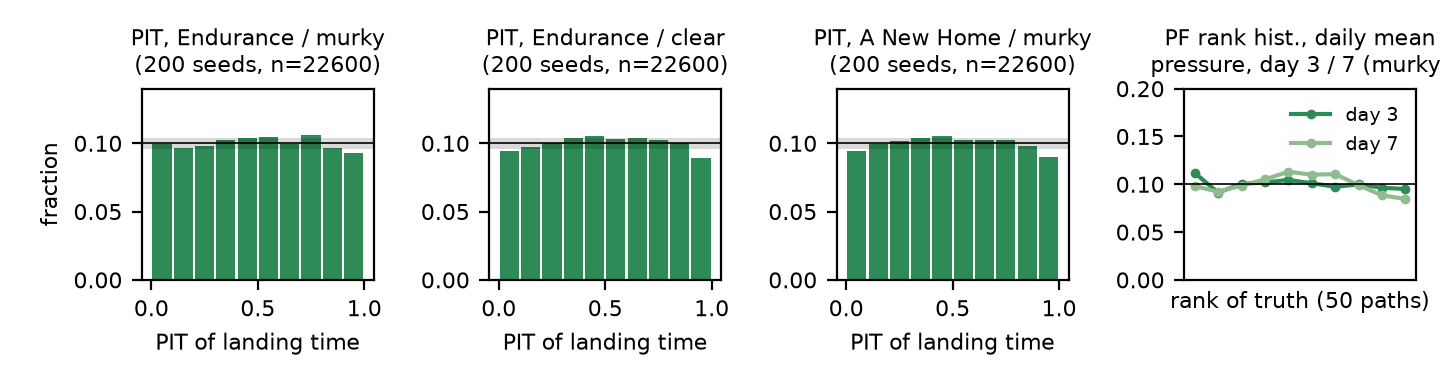
\includegraphics[width=0.72\textwidth]{figures/pf_pit_rank.png}
\caption{Particle-filter oracle self-check on 200 test seeds $\times$ 113
issue times per setting. Left three: randomised PIT of the realised landing
time over the 29 classes (grey band: 95\% sampling band around uniform).
Right: rank of the realised daily-mean pressure among the 50 oracle paths.}
\label{fig:pit}
\end{figure*}

\begin{table}[t]
\centering
\caption{Oracle sweep (30 validation seeds, Endurance/murky): 72-hour BSS vs.\
climatology / log loss by particle count $N$ and jitter (Lorenz units per
hour). Without re-seeding ($N{=}1024$, jitter 0.03): 0.92 / 0.60.}
\label{tab:pf}
\footnotesize
\begin{tabular}{lcccc}
\toprule
$N$ & 0.003 & \textbf{0.01} & 0.03 & 0.1 \\
\midrule
256 & -- & 0.85 / 0.92 & 0.92 / 0.63 & -- \\
1024 & 0.84 / 1.05 & \textbf{0.94 / 0.56} & 0.92 / 0.60 & 0.86 / 0.86 \\
4096 & 0.88 / 0.83 & 0.94 / 0.52 & 0.92 / 0.59 & -- \\
\bottomrule
\end{tabular}
\end{table}

%======================================================================
\section{Methods}\label{sec:methods}
%======================================================================
All learned models see the past 168 hours of precursors (pressure, trend,
wind speed, one-hot wind sector, animals, sky, storm flags, a validity mask;
16 features per hour) and six clock features (episode time, hours since the
last storm ended, whether a storm has occurred, whether one is under way,
hours left in it, scenario flag).

\paragraph*{Climatology} The training-set frequency of the 29 classes.

\paragraph*{Clock hazard} A lookup table keyed by the time since the last
storm ended (or the time left in the current storm, or the time since episode
start), in six-hour steps, fitted on training weather with additive smoothing.
Because storms last two days and are followed by a four-day refractory period,
and none lands before day 8, the clock alone has non-trivial skill; every
model is also scored relative to it.

\paragraph*{Bot rule} The clock table additionally keyed by the game's
scripted warning flag.

\paragraph*{GRU} A single-layer GRU~\cite{cho2014gru} (96 units) over the
history, concatenated with the clock features, followed by an MLP that outputs
29 logits; cross-entropy, AdamW, 16{,}000 steps of batch 256 at random issue
hours (about 1\,h on two CPU threads). Since at most one storm can land within
seven days, this categorical output is already a complete description of the
event; it is the strongest honest baseline for RQ1.

\paragraph*{Diffusion forecaster} A conditional denoising diffusion
model~\cite{ho2020ddpm} generates the next 168 hours of three channels:
normalised pressure, normalised wind speed and a storm flag in $\{-1,1\}$,
in the spirit of CSDI~\cite{tashiro2021csdi} (non-autoregressive,
whole-window). The condition is a strided 1-D convolutional encoding of the
history (168$\to$11 steps) concatenated with the clock features and the last
six hours verbatim, mapped by an MLP to a condition vector (96-d for v2,
256-d for v3). Two extra input channels give the denoiser the hour position
$1..168$ and a mask of the hours during which an ongoing storm is already
known to continue. Both denoisers below share a cosine noise
schedule~\cite{nichol2021improved}, the $v$-prediction
objective~\cite{salimans2022progressive} and deterministic DDIM
sampling~\cite{song2021ddim}. We use $T{=}200$ noise levels, weight the
loss on the storm-flag channel $\times3$ and clamp the predicted clean sample
per channel during sampling. Training uses AdamW (weight decay $10^{-4}$)
with a one-cycle learning-rate schedule, gradient clipping at norm 1 and
batches of 256 windows at random issue hours of the training seeds. The
denoising loss is evaluated at regular intervals on one fixed set of
2{,}048 validation windows, and we keep the checkpoint with the lowest
validation loss; no test seed is used to choose a model or a checkpoint.

\paragraph*{Diffusion v2 (U-Net)} Diffusion v2 has a convolutional denoiser.
The denoiser is a three-level 1-D
U-Net~\cite{ronneberger2015unet} (channels 32/48/64, residual blocks with
GroupNorm and FiLM~\cite{perez2018film} conditioning on the condition vector
plus a sinusoidal noise-level embedding; about $3\times10^5$ parameters).
It was first trained for 12{,}000 steps on CPU (learning rate
$3\times10^{-4}$, about 2.6\,h on four threads); that model, still
improving on validation, is the one in the ablation below. Trained unchanged
for 100{,}000 steps on a GPU, its validation loss reaches a noisy plateau
after about 60{,}000 steps (Fig.~\ref{fig:lc}); diffusion v2 in the main
results is the best validation checkpoint of that run (step \lcBestStep).

\paragraph*{Diffusion v3 (transformer)} The v3 denoiser treats each of the
168 future hours as one token: the three noisy channels and the two extra
channels of an hour are projected linearly to 160 dimensions and added to a
learned position embedding, followed by four transformer blocks with
five-head self-attention over all 168 hours and an MLP, and a linear output
layer (2.78\,M parameters). Each block, and the output layer, is conditioned on
the sum of the condition vector and an embedding of the noise level through
adaLN-zero~\cite{peebles2023dit}, which regresses the shift and scale of
each layer norm and a gate on each residual branch from the conditioning,
initialised so that every block starts as the identity function. Among three configurations of 2--3\,M parameters (this one and two wider
U-Nets with self-attention at the coarsest level), each trained for 100k steps
at learning rates $10^{-4}$, $3\times10^{-4}$ and $10^{-3}$, the rule fixed
before training (lowest validation loss) chose the transformer at $10^{-3}$,
by less than the noise of the validation plateau; all three reached a lower
validation loss than v2. It was then trained for 100k GPU steps from three
training seeds, each keeping its best validation checkpoint; main results
report the median over the three seeds with their range. The selection run
(seed 0) serves only as the reference of the marginal control, and the
secondary settings and the wind-noise ablation retrain seed 1.

\paragraph*{Sampling} In the main evaluation each diffusion forecast draws
\pathsDiff{} trajectories with \ddimSteps{} DDIM steps. The ablation, the
learning curve and the marginal control use 50 trajectories and 25 DDIM steps
on test seeds 220000--220059, and Table~\ref{tab:samples} varies the number
of trajectories.

\paragraph*{Landing readout} A sampled trajectory lands at the first hour at
which the storm flag turns on (and is not the continuation of a storm already
under way) and stays on for at least three hours; event probabilities are the
fractions of the sampled trajectories per class.

% S1-7 ablation (ml/forecast/out/ablation/summary_abl{A..D}.json, diff.BSS{72,168}_clim[0])
\newcommand{\ablABssSeventyTwo}{$-$0.40}
\newcommand{\ablABssOneSixtyEight}{$-$0.23}
\newcommand{\ablBBssSeventyTwo}{0.11}
\newcommand{\ablBBssOneSixtyEight}{0.06}
\newcommand{\ablCBssSeventyTwo}{0.68}
\newcommand{\ablCBssOneSixtyEight}{0.31}
\newcommand{\ablDBssSeventyTwo}{0.67}
\newcommand{\ablDBssOneSixtyEight}{0.32}
\paragraph*{What the v2 design fixed}
A first version without the position and known-remainder channels, trained
with $\epsilon$-prediction, did not know where it was in the window (with a
storm under way only 31\% of samples continued it; in calm, 23\% landed a
storm in the next hour) and had negative skill at every lead.
Table~\ref{tab:ablation} adds the v2 changes one at a time (one 12k-step run
each). The position and remainder channels fix this behaviour and lift the
skill just above climatology; almost all of the remaining gain comes from
$v$-prediction. Weighting the storm-flag loss $\times3$ does not change the
event skill measurably; we keep it so that v2 and v3 validation losses are
comparable. Longer training of v2 adds considerably more
(Section~\ref{sec:discussion}).

\begin{table}[t]
\centering
\caption{v1$\to$v2 ablation (Endurance/murky, test seeds 220000--220059, 12k training
steps, one training seed each, DDIM 25, 50 paths): BSS vs.\ climatology with
95\% seed-bootstrap intervals, and energy score of the daily paths (lower is
better). Each row adds one change to the row above; D is v2.}
\label{tab:ablation}
\small\setlength{\tabcolsep}{3pt}
\resizebox{\columnwidth}{!}{%
\begin{tabular}{llccc}
\toprule
 & change & BSS$_{72}$ & BSS$_{168}$ & ES \\
\midrule
A & v1 ($\epsilon$-pred.) & \ablABssSeventyTwo{} [$-$0.45, $-$0.36] & \ablABssOneSixtyEight{} [$-$0.27, $-$0.20] & 3.62 \\
B & + pos./remainder & \ablBBssSeventyTwo{} [0.08, 0.13] & \ablBBssOneSixtyEight{} [0.02, 0.09] & 3.32 \\
C & + $v$-pred. & \ablCBssSeventyTwo{} [0.66, 0.70] & \ablCBssOneSixtyEight{} [0.28, 0.33] & 2.14 \\
D & + flag $\times3$ (= v2) & \ablDBssSeventyTwo{} [0.65, 0.70] & \ablDBssOneSixtyEight{} [0.30, 0.34] & 2.23 \\
\bottomrule
\end{tabular}}
\end{table}

%======================================================================
\section{Metrics}\label{sec:metrics}
%======================================================================
For each lead $L\in\{12,24,48,72,96,120,144,168\}$\,h we compute the Brier
score of $P(\text{landing}\le L)$ and the Brier skill score
$\BSS = 1 - \mathrm{BS}/\mathrm{BS}_{\text{ref}}$ against climatology and
against the clock baseline. Over the ordered 29 classes we report the
categorical CRPS of the landing time (in hours), i.e.\ the ranked
probability score over the ordered classes, whose infinite-class limit is the
CRPS~\cite{hersbach2000}, the
log loss (probabilities floored at $10^{-4}$), the 1-Wasserstein distance to
the oracle's landing distribution (hours) and
$\mathrm{KL}(p_{\text{oracle}}\,\|\,p_{\text{model}})$. For trajectory
forecasts we compute the energy score~\cite{gneiting2007proper} and the
variogram score with $p{=}0.5$~\cite{scheuerer2015} on daily means (21
dimensions: pressure/5\,hPa, wind/3\,m/s, storm flag); the variogram score is
sensitive to wrong temporal correlation, which is what a per-lead marginal
model gets wrong. We also show reliability diagrams, and PIT and rank
histograms~\cite{hamill2001,gneiting2007calibration}. Confidence intervals are
95\% bootstrap intervals over test seeds (1{,}000 resamples).

%======================================================================
\section{RQ1 Results: Forecasting from Precursors}\label{sec:rq1}
%======================================================================
Main setting: Endurance, murky precursors, all 200 test seeds $\times$ 113
daily issue times, every method on the same seeds. Two diffusion models are
evaluated (Section~\ref{sec:methods}), each drawing \pathsDiff{} trajectories
per forecast with \ddimSteps{} DDIM steps: \emph{v2}, the U-Net at its best
validation checkpoint (step \lcBestStep{} of a 100{,}000-step run; the
12k-step model of the ablation is undertrained, see the discussion), and
\emph{v3}, the transformer denoiser trained from three training seeds. For v3
we report the median over the three training seeds and, in parentheses, their
range; intervals in square brackets are 95\% bootstrap intervals over test seeds.

\begin{table*}[t]
\centering
\caption{Brier skill score vs.\ climatology by lead time (Endurance/murky, 200 test seeds $\times$ 113 issue times; diffusion with \pathsDiff{} paths and \ddimSteps{} DDIM steps). Square brackets: 95\% CIs over test seeds at 72\,h and 168\,h. Diffusion v3: median of three training seeds, range over the seeds in parentheses.}
\label{tab:bss}
\setlength{\tabcolsep}{4pt}
\begin{tabular}{lcccccccc}
\toprule
Method & 12h & 24h & 48h & 72h & 96h & 120h & 144h & 168h \\
\midrule
Clock hazard & \bssRowClock \\
Bot rule & \bssRowBot \\
GRU & \bssRowGru \\
Diffusion v2 (U-Net) & \bssRowDiffTwo \\
Diffusion v3 (transformer) & \bssRowDiffThree \\
\midrule
PF oracle & \bssRowPf \\
\bottomrule
\end{tabular}
\end{table*}

\begin{table}[t]
\centering
\caption{Landing-time and trajectory scores (Endurance/murky, 200 test seeds $\times$ 113 issue times). Lower is better. CRPS and W1 to the oracle in hours. ES/VS rows for climatology, clock and GRU use the analogue path generators of Section~\ref{sec:rq1} with \pathsAnalogue{} paths per forecast; diffusion uses \pathsDiff{} paths, the PF oracle its 50 paths. Diffusion v3: median of three training seeds.}
\label{tab:scores}
\setlength{\tabcolsep}{3pt}
\begin{tabular}{lcccccc}
\toprule
Method & CRPS & LogL & W1$_\text{PF}$ & KL & ES & VS \\
\midrule
Climatology & \scRowClim \\
Clock & \scRowClock \\
Bot rule & \scRowBot \\
GRU (+ analogue paths) & \scRowGru \\
Diffusion v2 & \scRowDiffTwo \\
Diffusion v3 & \scRowDiffThree \\
\midrule
PF oracle & \scRowPf \\
\bottomrule
\end{tabular}
\\[2pt]{\footnotesize ES/VS: energy and variogram scores on 21-d daily means (bootstrap 95\% CIs are within $\pm$\esCiMax{} and $\pm$\vsCiMax{} for every row; v3 range over training seeds: ES \esDiffThreeRange, VS \vsDiffThreeRange). The sample estimate of the energy score is biased upwards by about $\E\|X-X'\|/(2M)$ for $M$ paths, so the oracle's 50-path ES is slightly pessimistic relative to the 200-path rows.}
\end{table}

\begin{figure}[t]
\centering
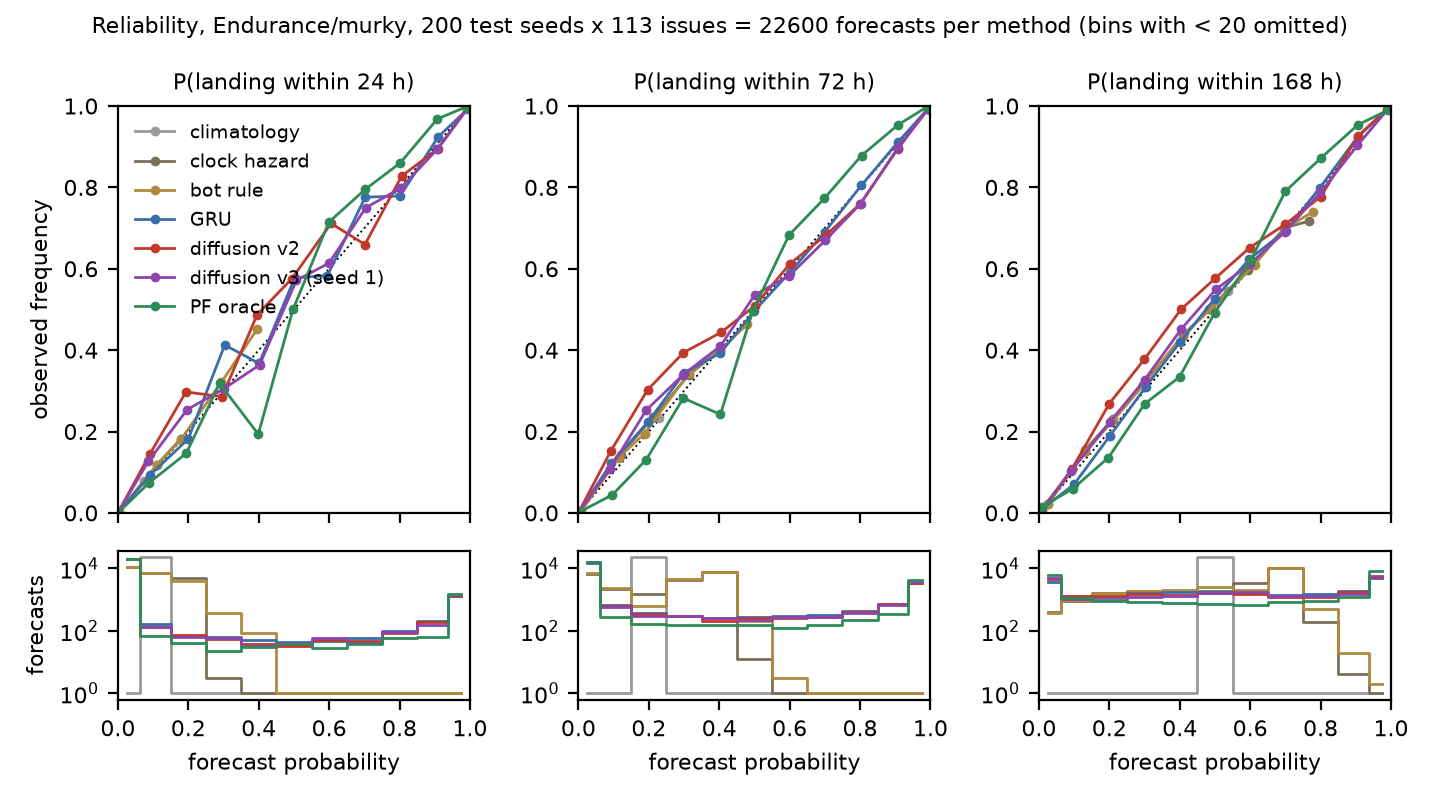
\includegraphics[width=0.82\columnwidth]{figures/reliability_all.png}
\caption{Reliability of $P(\text{landing within }L)$ for $L=24/72/168$\,h,
all methods on the same 200 test seeds $\times$ 113 issues (Endurance/murky;
diffusion v2 and v3 training seed 1).
Bottom: number of forecasts per probability bin (log scale); bins with fewer
than 20 forecasts are omitted. The PF's dips at 72\,h fall in bins holding
fewer than 100 forecasts.}
\label{fig:rel}
\end{figure}

\paragraph*{Precursors carry most of the information}
The clock and the scripted warning rule reach only $\bssClockSeventyTwo$ and
$\bssBotSeventyTwo$ skill at 72\,h (the rule adds at most
$\bssBotOverClockMax$ over the clock at any lead), while the oracle, using the
same precursors, reaches $\bssPfSeventyTwo$ at 72\,h and
$\bssPfOneSixtyEight$ at 168\,h (Table~\ref{tab:bss}).
Relative to the clock, the 72/168\,h skill is
$\bssClockPfSeventyTwo/\bssClockPfOneSixtyEight$ for the oracle,
$\bssClockGruSeventyTwo/\bssClockGruOneSixtyEight$ for the GRU,
$\bssClockDiffTwoSeventyTwo/\bssClockDiffTwoOneSixtyEight$ for v2 and
$\bssClockDiffThreeSeventyTwo/\bssClockDiffThreeOneSixtyEight$ for v3. Skill
decays smoothly with lead time, consistent with the roughly 1.6-day
error-doubling time of the dynamics.

\paragraph*{Event forecasts: GRU and diffusion}
On the landing event the GRU and the two diffusion models are close to one
another and all well short of the oracle: 72-hour skill $\bssGruSeventyTwo$,
$\bssDiffTwoSeventyTwo$ and $\bssDiffThreeSeventyTwo$ (GRU, v2, v3),
landing-time CRPS \crpsGru{}, \crpsDiffTwo{}
and \crpsDiffThree{}\,h (oracle \crpsPf\,h; Tables~\ref{tab:bss}
and~\ref{tab:scores}). The spread over v3's training seeds is far smaller than
the test-seed intervals. The GRU is much cheaper: one forward pass gives the
29 classes, whereas each diffusion forecast needs \pathsDiff{} trajectories of
\ddimSteps{} denoising steps. Diffusion event probabilities are fractions of
\pathsDiff{} samples (empty classes floored at $10^{-4}$), which affects the
log loss (GRU \llGru, v2 \llDiffTwo, v3 \llDiffThree).

\paragraph*{Sample count}
To separate this granularity from model error, v3 (training seed~1) drew
500 trajectories per forecast on test seeds 220000--220059, read out from the
first 50, 200 and all 500 paths (Table~\ref{tab:samples}). The log loss falls
from \llNFifty{} to \llNTwoHundred{} and \llNFiveHundred, as binomial
sampling from the 500-path probabilities alone predicts (\llPredNFifty{} and
\llPredNTwoHundred), mostly through forecasts in which no path reached the
observed class; the 72\,h BSS stays at \bssNFifty--\bssNFiveHundred. The
\pathsDiff-path readout of the main tables thus leaves a granularity effect of
about \dllNTwoHundred{} on the log loss and none of consequence on the BSS.

\begin{table}[t]
\centering
\caption{Sample count of the diffusion readout (v3, training seed~1;
Endurance/murky, test seeds 220000--220059 $\times$ 113 issue times; 50 and 200 are
the first paths of the same 500). ``Sampling only'': expected log loss when
$k$ outcomes are drawn binomially from the 500-path probabilities.
``Floored'': forecasts in which no path reached the observed class.
BSS$_{72}$ corr.: Brier score minus $p(1-p)/(k-1)$. 95\% intervals over
test seeds: log loss as shown; BSS$_{72}$ \bssNFiftyCI, \bssNTwoHundredCI{} and \bssNFiveHundredCI.}
\label{tab:samples}
\setlength{\tabcolsep}{2pt}
\footnotesize
\begin{tabular}{rccccc}
\toprule
Paths & Log loss & Sampling only & Floored (\%) & BSS$_{72}$ & BSS$_{72}$ corr. \\
\midrule
50 & \llNFifty{} \llNFiftyCI & \llPredNFifty & \floorPctNFifty & \bssNFifty & \bssDbNFifty \\
200 & \llNTwoHundred{} \llNTwoHundredCI & \llPredNTwoHundred & \floorPctNTwoHundred & \bssNTwoHundred & \bssDbNTwoHundred \\
500 & \llNFiveHundred{} \llNFiveHundredCI & \llPredNFiveHundred & \floorPctNFiveHundred & \bssNFiveHundred & \bssDbNFiveHundred \\
\bottomrule
\end{tabular}
\end{table}

\paragraph*{Calibration and sharpness}
The reliability curves of the GRU and both diffusion models track the
diagonal closely at all three leads (Fig.~\ref{fig:rel}; v2 is slightly low
between about 0.1 and 0.4 at 72 and 168\,h), so the remaining gap to the
oracle is one of sharpness rather than calibration. In the case of
Fig.~\ref{fig:example} (landing \exLandHours\,h after issue) the probability
that a storm is under way peaks at \exPeakPf{} for the oracle and
\exPeakDiff{} for v3, v3's rising a few hours earlier, and v3's pressure paths
spread more widely around the pre-landing minimum.

\paragraph*{Economic value}
In the static cost--loss model (Section~\ref{sec:related}) a user who pays
$C$ to protect against a loss $L$ protects whenever the forecast probability
is at least $C/L$; $V$ is the expense saved over the better of always and
never protecting, relative to perfect knowledge (Fig.~\ref{fig:value}). At
72\,h and $C/L=0.1$ the clock and the warning rule reach \vcClockSeventyTwo{}
and \vcBotSeventyTwo, the GRU \vcGruSeventyTwo{} \vcGruSeventyTwoCI, v2
\vcDiffTwoSeventyTwo{} \vcDiffTwoSeventyTwoCI, v3 \vcDiffThreeSeventyTwo{}
(seeds \vcDiffThreeSeventyTwoRange) and the oracle \vcPfSeventyTwo{}
\vcPfSeventyTwoCI; the learned curves and the oracle peak at the base rate
(\vcBaseRateSeventyTwo) at \vcGruPeak, \vcDiffTwoPeak, \vcDiffThreePeak{} and
\vcPfPeak. At 168\,h ($C/L=0.1$) the values are \vcGruOneSixtyEight,
\vcDiffTwoOneSixtyEight, \vcDiffThreeOneSixtyEight{} and
\vcPfOneSixtyEight. Being calibrated, the learned forecasts lose at most 0.023
of value at face value for $C/L\le0.9$; the oracle at 168\,h does worse than
always protecting at $C/L=0.01$ ($V=-0.15$), because 1.3\% of the windows it
gives below 0.01 contain a landing.

\begin{figure*}[t]
\centering
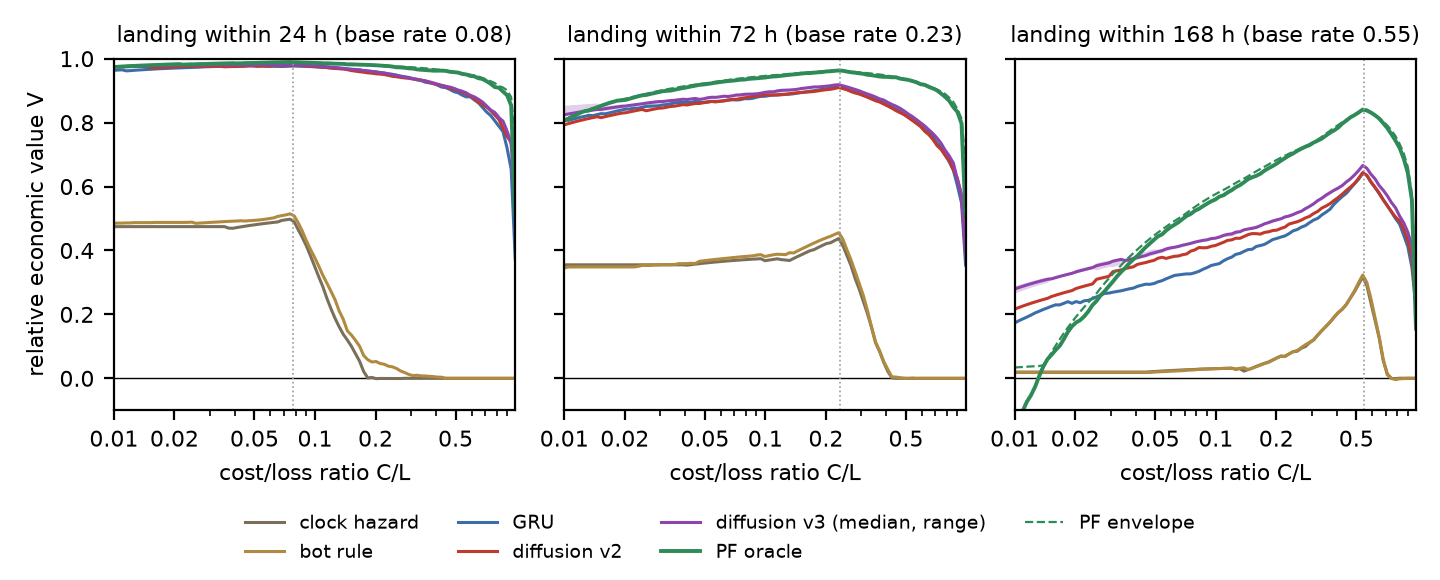
\includegraphics[width=0.64\textwidth]{figures/value_curve.png}
\caption{Relative economic value $V$ of $P(\text{landing within }L)$ against
the cost/loss ratio $C/L$, $L=24/72/168$\,h (Endurance/murky, 200 test seeds
$\times$ 113 issues). Each user protects when the forecast probability is at
least $C/L$; dashed: the oracle's envelope (best threshold for each $C/L$).
Diffusion v3: median of three training seeds, shaded range over the seeds.
Dotted vertical line: base rate.}
\label{fig:value}
\end{figure*}

\paragraph*{What diffusion adds: coherent scenarios}
Unlike the event classifiers, the diffusion models and the oracle produce
\emph{joint} seven-day trajectories that a planner can consume. The oracle's
energy and variogram scores (\esPf{} and \vsPf) bound what is achievable;
diffusion v2 reaches \esDiffTwo{} and \vsDiffTwo, v3 \esDiffThree{} and
\vsDiffThree{}, with training-seed ranges \esDiffThreeRange{} and \vsDiffThreeRange. As references, three generators draw \pathsAnalogue{} real 168-hour training
futures per issue: \emph{climatology} (same episode hour), \emph{clock
analogues} (same clock state) and \emph{GRU + analogues} (a landing class
drawn from the GRU forecast, then a future with that first-landing class and,
where possible, the same clock state; \pbFallback{} of \pbDraws{} draws fell
back to class only). They score ES \esClimPaths, \esClockPaths{} and
\esGruPaths{} and VS \vsClimPaths, \vsClockPaths{} and \vsGruPaths. Much of
the observable path is implied by the landing time (storm flag, storm-time
wind jump), so real weather behind a good event forecast is a strong
reference; diffusion instead conditions every hour on the history.

\begin{figure}[t]
\centering
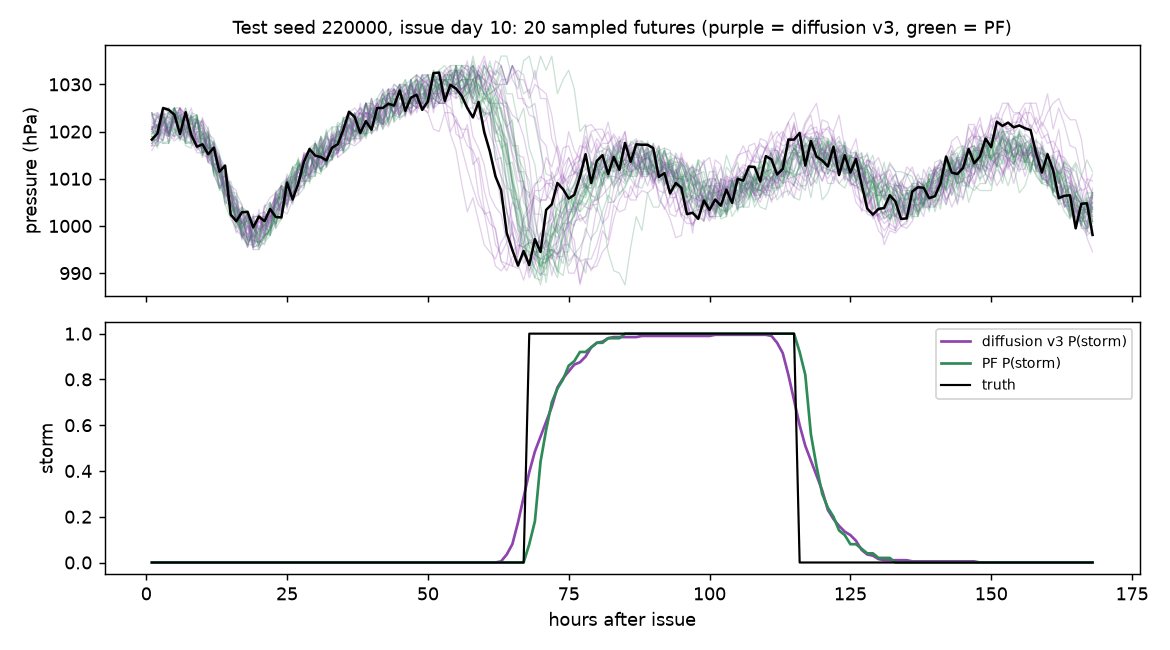
\includegraphics[width=0.78\columnwidth]{figures/e1_example_endurance_murky.png}
\caption{Test seed \exSeed, issued on day \exIssueDay. Top: 20 sampled pressure futures
(purple: diffusion v3, training seed 1; green: oracle; black: truth). Bottom:
probability that a storm is under way (diffusion: fraction of its
\pathsDiff{} paths; oracle: of its 50 paths).}
\label{fig:example}
\end{figure}

\paragraph*{Is the joint structure real? A marginal control}
\newcommand{\bssMargSeventyTwo}{0.86}
\newcommand{\esMarg}{1.51}
\newcommand{\vsMarg}{16.7}
\newcommand{\esDiffOnMargSet}{1.30}
\newcommand{\vsDiffOnMargSet}{17.4}
To test whether the joint structure matters, we take the v3 selection run
(training seed 0) and restrict attention to the diagonal, so that every hour
is sampled independently given the history, adding a per-hour output channel
``the next landing has happened by the end of this 6-hour bin'' from which
event probabilities are read directly; everything else is unchanged and the
control is trained once. As a diagnostic we also permute the joint model's 50
samples independently at every hour, which keeps its per-hour marginals and
removes its joint structure (Table~\ref{tab:marginal}).

\begin{table}[t]
\centering
\caption{Marginal control vs.\ joint diffusion (transformer denoiser, Endurance/murky, test seeds 220000--220059, DDIM 25, 50 paths; 95\% seed-bootstrap CIs). BSS vs.\ climatology (higher is better); ES/VS on 21-d daily means (lower is better).}
\label{tab:marginal}
\setlength{\tabcolsep}{2pt}
\resizebox{\columnwidth}{!}{%
\begin{tabular}{lcccc}
\toprule
Model & BSS 72h & BSS 168h & ES & VS \\
\midrule
Joint diffusion & \mcRowJoint \\
Marginal control & \mcRowMarg \\
Joint, hours permuted & \mcRowShuf \\
\bottomrule
\end{tabular}}
\end{table}

On events the control lies slightly above the joint model (paired
differences \mcBssSeventyTwo{} \mcBssSeventyTwoCI{} at 72\,h,
\mcBssOneSixtyEight{} \mcBssOneSixtyEightCI{} at 168\,h). The path scores
order the models differently: the control's energy score is higher (\mcEs{}
\mcEsCI, \mcEsRelPct\%) and its variogram score lower (\mcVs{} \mcVsCI).
Permuting the joint model's hours raises both of its scores (ES \mcEsShuf{}
\mcEsShufCI, VS \mcVsShuf{} \mcVsShufCI), so its cross-hour structure is
real, while the control's per-hour marginals are sharper (\mcEsMargShuf{} in
ES and \mcVsMargShuf{} in VS relative to the permuted model). On the
variogram score, which targets pairwise structure, the sharper marginals
outweigh the missing dependence; on the energy score they do not. With one
training run per model, whether joint generation improves the paths depends
on the path score.

\paragraph*{Clear signs and the scripted scenario}
Table~\ref{tab:secondary} reports the secondary settings (200 test seeds).
Clearer pressure readings raise GRU and oracle skill; in \emph{A New Home} the
great storm's calendar window makes the clock more informative, and the
learned models and the oracle remain well above it. Diffusion v3, trained once
per setting (training seed 1), places between the GRU and the oracle in both
settings at both leads, and the landing-time CRPS follows the same order
(clear: \secClearGruCrps, \secClearDiffCrps{} and \secClearPfCrps\,h;
\emph{A New Home}: \secHomeGruCrps, \secHomeDiffCrps{} and \secHomePfCrps\,h).
The paths' energy score is \secClearDiffEs{} for diffusion and
\secClearPfEs{} for the oracle with clear signs, \secHomeDiffEs{} and
\secHomePfEs{} in \emph{A New Home}.

\begin{table}[t]
\centering
\caption{Secondary settings, 72\,h / 168\,h BSS vs.\ climatology (200 test seeds).}
\label{tab:secondary}
\setlength{\tabcolsep}{3pt}
\begin{tabular}{lcccc}
\toprule
Setting & Clock & GRU & Diffusion & PF oracle \\
\midrule
Endurance / murky & \bssClockSeventyTwo{} / \bssClockOneSixtyEight & \bssGruSeventyTwo{} / \bssGruOneSixtyEight & \bssDiffThreeSeventyTwo{} / \bssDiffThreeOneSixtyEight$^{*}$ & \bssPfSeventyTwo{} / \bssPfOneSixtyEight \\
% BEGIN e18-rows (generated by ml/forecast/windows/secondary.py tex from ml/forecast/out/eval200/summary_{endurance_clear,a_new_home_murky}.json; do not edit)
Endurance / clear & 0.16 / 0.15 & 0.91 / 0.68 & 0.93 / 0.76 & 0.96 / 0.86 \\
A New Home / murky & 0.26 / 0.39 & 0.84 / 0.66 & 0.85 / 0.70 & 0.95 / 0.86 \\
% END e18-rows
\bottomrule
\end{tabular}
\\[2pt]{\footnotesize $^{*}$Diffusion v3, median of three training seeds (Table~\ref{tab:bss}); in the secondary settings, one training seed (seed 1).}
\end{table}

%======================================================================
\section{RQ2: The Value of Foresight}\label{sec:rq2}
%======================================================================
\subsection{Protocol}
All agents are PPO~\cite{schulman2017ppo} actor--critic MLPs (two tanh layers
of 64 units for policy and value, no recurrence) with action masking, trained
by our distributed PPO implementation on the Rust simulator. Every rung is
fine-tuned from the same checkpoint (the final model of our curriculum's stage
11) for 200M environment steps on HARDCORE, chaotic weather, murky precursors,
episodes capped at 120 days (about nine storms). New observation inputs are
zero-initialised. Hyperparameters: $\gamma{=}0.9995$, GAE $\lambda{=}0.98$,
learning rate $3\times10^{-4}$, 4 epochs per update with minibatch 4096,
clip 0.2, entropy coefficient 0.01; each round collects 10\,s of experience
from 8 Rust environments (about $10^5$ steps). The ladder is:
\begin{enumerate}
\item \textbf{No signs}: the base 128-d observation (camp state, in-storm flag).
\item \textbf{Raw signs}: + six current precursor readings (134-d):
pressure deviation $(p-1013\,\text{hPa})/30$, 24-hour pressure trend$/30$\,hPa,
wind sector$/7$, wind speed$/25$\,m/s, animal stage$/2$ and sky state$/3$.
\item \textbf{Signs + forecast}: + six forecast features from the frozen RQ1
GRU (Endurance, murky; 140-d): $P(\text{landing}\le L)$ for
$L\in\{24,48,72,120,168\}$\,h and the expected hours to the next landing$/240$
(no landing within 168\,h counted as 240\,h). The GRU runs online in the
environment wrapper on the last 168\,h of the agent's own readings and the
observable storm bookkeeping (inputs checked identical to its training
features on 4{,}262 hours), re-issued every 3 game hours; on held-out RL
episodes its $P(\le72\,\text{h})$ has BSS$_{72}$ 0.85 over calm hours, in line
with Table~\ref{tab:bss}. Rung 3a is trained three times like the other rungs
(13.5--14.9\,h per run).

\emph{Rungs 3b and 3a$^{\prime}$.} Sampling the diffusion model inside
every rollout step is too slow for PPO, so rung 3b reads the same six
features from a pre-computed table: one forecast per game day, issued at
\ebIssueHour{} and held until the next issue, from diffusion v3 (training seed
1, \ebTableDdim{} DDIM steps, \ebTablePaths{} paths) for a pool of
\ebTableSeeds{} training seeds and the \ebTableSeeds{} evaluation seeds. The
matched control 3a$^{\prime}$ uses a table of the same shape from the frozen
GRU, so 3b and 3a$^{\prime}$ differ only in the forecaster behind the daily
values (simulator, start, hyperparameters and budget are the same). Each is
trained three times on the laptop's CPU, with rounds sized to rung 3a's
average of \ebStepsPerRound{} steps.
\item \textbf{Oracle date}: signs + the true hours to the next landing
($\min(h/240,1)$) and its tier (136-d); an upper bound.
\end{enumerate}
Because the policy has no memory, rung 2 can only use the current readings
and the 24-hour trend; rung 3 supplies the history integration. All new input
columns start at zero, so every rung starts as the same policy.

\paragraph*{Storm-focused metrics} Days survived, the planned measure, turned
out to be a poor measure of foresight because most episodes end by exile or a
furnace explosion. We therefore measure foresight on every storm a colony
\emph{reaches} (landing with people alive): deaths during the storm, whether
anyone died, and deaths per 100 colonists at landing. Weather depends only on
the seed, so storm $k$ of seed $s$ is the same storm for every agent
(checked on all 3{,}572 shared storms) and paired comparisons use the storms
both agents reached. Each rung is trained three times; we report the mean over
runs with its spread, and paired differences pooled over runs with 95\%
bootstrap CIs over evaluation seeds, which cover evaluation noise only;
training variance shows in the per-run values and in how many runs have a
per-run CI below or above zero.

\paragraph*{Implicit-forecast probe}
We record the hidden activations of the rung-2 policy and value networks on
held-out episodes and fit linear probes~\cite{alain2016probes}, a ridge
regression (and a logistic probe for ``landing within 72\,h''), to the oracle's hours-to-landing, then compare the
held-out $R^2$/Brier skill with (i) the same probe on the raw input
observation, which controls for information that is linearly available in the
input, and (ii) the particle filter, which is the ceiling given the full
history. A hidden-state probe that clearly exceeds the input-only probe would
indicate a learned forecast-like feature. We also fit a $2\times128$ MLP on
the raw observation (early-stopped), which approximates the best memoryless
function of the input. Probes use the greedy rollouts on seeds
300000--300199, calm hours only (about 190{,}000 per agent), split by seed
(140 train / 60 test).

\subsection{Results}\label{sec:rq2res}
We evaluate the final checkpoint of each rung, the common stage-11 starting
checkpoint and the game's scripted bot on 1{,}000 held-out seeds
(300000--300999) under the training conditions, with the simulator the
policies were trained on (the Rust module of the frozen commit
\texttt{4195eb6}; a 600-episode re-run against a frozen copy of its data
reproduced every episode exactly). We report greedy (arg-max) actions and
actions sampled from the policy, as in training. Storm deaths are deaths in
hours during which a storm was under way.

\paragraph*{Days survived do not separate the rungs} All rungs improve on the
starting checkpoint (37.1 days, greedy) and the scripted bot (20.6 days), but
between rungs the differences are small next to the spread between training
runs (Table~\ref{tab:storms}): greedy, 49.3 days without signs, 47.1 with raw
signs and 53.3 with the oracle date; raw signs minus no signs is $+2.9$,
$-11.8$ and $+2.3$ days in the three runs, and within run 1 mean survival
moves by up to 17 days between the last six checkpoints
(Table~\ref{tab:ladder}: run 1).

\paragraph*{Exile, not storms, ends the episodes} Storms cause only 16--19\%
of all deaths. Most episodes end with people alive because the camp exiles
its leader after a failed discontent/hope ultimatum (45--76\% of greedy
episodes, 82--91\% of sampled episodes in all but two runs); furnace
explosions end 1--35\% and die-outs 11--52\%. The exceptions are no-signs runs
2 and 3, which with sampled actions reach the 120-day cap in 40\% and 32\% of
episodes (others $\le$1\%) with larger, better-fed, less discontented
colonies. This colony-management strategy, unrelated to the weather inputs,
is the largest effect in the ladder, so we measure foresight per storm.

\paragraph*{Per storm reached: oracle date vs.\ raw signs and no signs}
Table~\ref{tab:storms} and Fig.~\ref{fig:ladder} condition on storms reached
(3.3--4.5 per episode for the PPO rungs). With greedy actions the oracle-date
agent loses 2.07 people per storm, against 2.16 without signs and 2.76 with
raw signs. Oracle minus raw signs is $-0.78$ [$-0.88$, $-0.66$], with per-run
CIs below zero in all three runs for all three storm metrics, and keeps its
sign in every run with sampled actions ($-0.29$ [$-0.39$, $-0.20$]). Oracle
minus no signs is $-0.25$ [$-0.35$, $-0.14$] greedy (all runs agree in sign)
but $+0.29$ [0.21, 0.38] sampled, decided by no-signs runs 2 and 3, whose
larger, better-fed colonies lose only 0.85--1.00 people per storm. Raw signs
give no reliable benefit over no signs ($+0.46$ [0.35, 0.58] greedy, $+0.44$
[0.35, 0.53] sampled). Losses hardly depend on the severity tier
(Fig.~\ref{fig:ladder}, right).

\paragraph*{Rung 3a: a GRU forecast as input}
With greedy actions the 3a agent loses 1.62 people per storm (runs
1.10--1.92). 3a minus raw signs is $-1.26$ [$-1.38$, $-1.15$] (runs $-0.90$,
$-2.24$, $-0.65$; per-run CIs below zero for all three metrics), and 3a minus
no signs $-0.78$ [$-0.89$, $-0.67$] (3/3 runs). With sampled actions the
difference to raw signs remains ($-0.45$ [$-0.54$, $-0.36$]; two runs below
zero, one above), while against no signs deaths per storm do not separate
($+0.07$ [$-0.01$, 0.16]). Oracle minus 3a is $+0.53$ [0.45, 0.63] greedy: the
oracle inputs bound the information about the next landing, not what PPO
learns from them in 200M steps. Days survived vary most between runs (44.8,
84.1 and 55.8, greedy), so pooled days are not evidence for the forecast.

\paragraph*{Rungs 3b and 3a$^{\prime}$: daily diffusion and daily GRU forecasts}
With greedy actions the 3b agent loses \ebFcdDeathsG{} people per storm (runs
\ebFcdDeathsGRuns) and the 3a$^{\prime}$ agent \ebFcgDeathsG{} (runs
\ebFcgDeathsGRuns). On the storms both reached, 3b minus 3a$^{\prime}$ is
\ebFcdFcgDeathsG{} deaths per storm \ebFcdFcgDeathsGCI{} (runs
\ebFcdFcgDeathsGRuns; per-run CI above zero in \ebFcdFcgDeathsGAbove, below
in \ebFcdFcgDeathsGBelow) and \ebFcdFcgDeathsS{} \ebFcdFcgDeathsSCI{} with
sampled actions (runs \ebFcdFcgDeathsSRuns). The runs differ in sign: 3b run
3 loses the fewest people per storm of the six runs and reaches the 120-day
cap in \ebFcdCapGMax\% of its greedy episodes (the colony-management pattern
seen before), while 3b runs 1 and 2 lose more than every 3a$^{\prime}$ run.
Against rung 3a, 3b minus 3a is \ebFcdFcDeathsG{} \ebFcdFcDeathsGCI{}
greedy, again with runs of both signs. With the spread between 3b runs larger
than the pooled difference, three runs cannot order the two forecasters as
policy inputs.

\paragraph*{Checkpoint drift (run 1)} Over the last six checkpoints of run 1
(greedy), deaths per storm are $2.56\pm0.47$ (no signs), $2.50\pm0.27$ (raw
signs) and $2.25\pm0.24$ (oracle); the oracle--no-signs CI in P(any death)
lies below zero at five of six checkpoints, while the other two differences
flip sign.

\paragraph*{Preparation at landing} The agents do not prepare by stockpiling:
every PPO colony holds far more coal than a storm needs (median 710--1{,}080
hours of furnace burn vs.\ about 49\,h of storm; coal ran short in $\le$4\% of
storms vs.\ 95\% for the bot), and the furnace was raised in the 48\,h before
landing in only 9--13\% of storms for every rung. The value of the date shows
up as fewer deaths per storm, not as visible anticipatory actions.

\begin{figure*}[t]
\centering
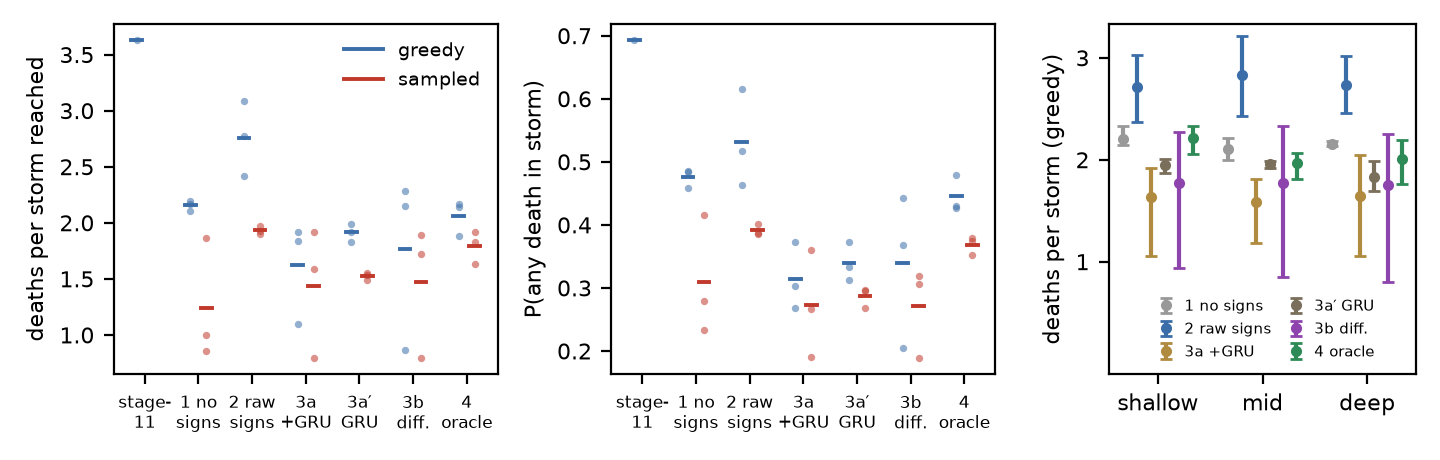
\includegraphics[width=0.64\textwidth]{figures/e0_storms.png}
\caption{Storm-focused E0 metrics, conditioned on storms reached (1{,}000
held-out seeds, final checkpoints, three training runs per rung). Rungs 3a$^{\prime}$ and 3b
read once-daily GRU and diffusion forecasts. Left, middle:
deaths per storm and probability that anyone dies; dots: the three runs; bars:
their mean; greedy and sampled actions. Right: deaths per storm by severity
tier (greedy), mean and range over runs.}
\label{fig:ladder}
\end{figure*}

\begin{table}[t]
\centering
\caption{Storm-focused ladder (HARDCORE, murky), per storm reached, 1{,}000 held-out seeds, final checkpoints, three training runs per rung. Top: mean $\pm$ s.d.\ over runs. Paired: difference on the storms (episodes, for days) both agents reached, pooled over runs, [95\% CI over evaluation seeds]; in brackets below, the number of runs whose own paired CI lies below / above zero. Stage-11 start and bot: one checkpoint. 3a$^{\prime}$ and 3b: once-daily GRU and diffusion forecast tables, otherwise identical.}
\label{tab:storms}
\setlength{\tabcolsep}{2pt}
\resizebox{\columnwidth}{!}{\begin{tabular}{lccccc}
\toprule
 & Storms/ep. & Deaths / storm & P(any death) & Deaths / 100 & Days \\
\midrule
\multicolumn{6}{l}{\emph{Greedy}} \\
Stage-11 start & 2.50 & 3.63 & 0.69 & 19.1 & 37.1 \\
1 No signs & 3.49 & 2.16 $\pm$ 0.05 & 0.48 $\pm$ 0.02 & 8.9 $\pm$ 0.7 & 49.3 $\pm$ 4.1 \\
2 Raw signs & 3.33 & 2.76 $\pm$ 0.34 & 0.53 $\pm$ 0.08 & 12.3 $\pm$ 1.8 & 47.1 $\pm$ 9.7 \\
3a Signs + GRU & 4.49 & 1.62 $\pm$ 0.45 & 0.31 $\pm$ 0.05 & 6.2 $\pm$ 2.2 & 61.6 $\pm$ 20.3 \\
% BEGIN e0b-storms-greedy (generated by ml/forecast/figures_paper.py storms3b from ml/forecast/out/storm_seeds_*.json; do not edit)
3a$^{\prime}$ Signs + daily GRU & 4.29 & 1.92 $\pm$ 0.08 & 0.34 $\pm$ 0.03 & 8.0 $\pm$ 1.5 & 59.1 $\pm$ 3.3 \\
3b Signs + diffusion & 3.90 & 1.77 $\pm$ 0.78 & 0.34 $\pm$ 0.12 & 7.1 $\pm$ 3.2 & 54.4 $\pm$ 10.0 \\
% END e0b-storms-greedy
4 Oracle date & 3.85 & 2.07 $\pm$ 0.16 & 0.45 $\pm$ 0.03 & 7.8 $\pm$ 1.2 & 53.3 $\pm$ 5.6 \\
Scripted bot & 1.17 & 1.71 & 0.73 & 33.5 & 20.6 \\
\multicolumn{6}{l}{\emph{Sampled}} \\
1 No signs & 4.75 & 1.24 $\pm$ 0.54 & 0.31 $\pm$ 0.09 & 3.9 $\pm$ 1.9 & 64.9 $\pm$ 16.5 \\
2 Raw signs & 3.41 & 1.93 $\pm$ 0.04 & 0.39 $\pm$ 0.01 & 5.6 $\pm$ 0.3 & 48.4 $\pm$ 0.5 \\
3a Signs + GRU & 4.16 & 1.43 $\pm$ 0.57 & 0.27 $\pm$ 0.08 & 4.7 $\pm$ 2.4 & 57.7 $\pm$ 23.6 \\
% BEGIN e0b-storms-sample (generated by ml/forecast/figures_paper.py storms3b from ml/forecast/out/storm_seeds_*.json; do not edit)
3a$^{\prime}$ Signs + daily GRU & 3.90 & 1.53 $\pm$ 0.03 & 0.29 $\pm$ 0.02 & 4.3 $\pm$ 0.3 & 54.4 $\pm$ 0.6 \\
3b Signs + diffusion & 4.01 & 1.47 $\pm$ 0.59 & 0.27 $\pm$ 0.07 & 4.5 $\pm$ 1.6 & 55.8 $\pm$ 9.4 \\
% END e0b-storms-sample
4 Oracle date & 3.79 & 1.80 $\pm$ 0.14 & 0.37 $\pm$ 0.01 & 5.3 $\pm$ 0.6 & 53.0 $\pm$ 1.9 \\
\midrule
\multicolumn{6}{l}{\emph{Paired, greedy}} \\
2$-$1 & & $+$0.46 [0.35, 0.58] & $+$0.025 [0.008, 0.042] & $+$2.2 [1.6, 2.7] & $-$2.2 [$-$3.2, $-$1.1] \\
 & & (0/2) & (1/2) & (0/2) & (1/2) \\
4$-$1 & & $-$0.25 [$-$0.35, $-$0.14] & $-$0.063 [$-$0.079, $-$0.046] & $-$1.9 [$-$2.4, $-$1.4] & $+$4.0 [2.9, 5.0] \\
 & & (2/0) & (3/0) & (3/0) & (0/3) \\
4$-$2 & & $-$0.78 [$-$0.88, $-$0.66] & $-$0.092 [$-$0.107, $-$0.075] & $-$4.4 [$-$4.9, $-$3.9] & $+$6.2 [5.3, 7.1] \\
 & & (3/0) & (3/0) & (3/0) & (0/2) \\
3a$-$2 & & $-$1.26 [$-$1.38, $-$1.15] & $-$0.234 [$-$0.250, $-$0.218] & $-$5.5 [$-$6.0, $-$5.1] & $+$14.5 [13.4, 15.5] \\
 & & (3/0) & (3/0) & (3/0) & (1/1) \\
3a$-$1 & & $-$0.78 [$-$0.89, $-$0.67] & $-$0.199 [$-$0.216, $-$0.183] & $-$3.1 [$-$3.6, $-$2.7] & $+$12.3 [11.1, 13.5] \\
 & & (3/0) & (3/0) & (2/0) & (0/2) \\
4$-$3a & & $+$0.53 [0.45, 0.63] & $+$0.149 [0.135, 0.164] & $+$1.4 [1.0, 1.8] & $-$8.3 [$-$9.4, $-$7.3] \\
 & & (0/2) & (0/3) & (1/2) & (1/2) \\
% BEGIN e0b-pairs-greedy (generated by ml/forecast/figures_paper.py storms3b from ml/forecast/out/storm_seeds_*.json; do not edit)
3b$-$3a$^{\prime}$ & & $+$0.22 [0.11, 0.32] & $+$0.043 [0.028, 0.058] & $+$1.0 [0.5, 1.5] & $-$4.7 [$-$5.9, $-$3.6] \\
 & & (1/2) & (1/2) & (1/2) & (2/1) \\
3b$-$3a & & $+$0.24 [0.14, 0.34] & $+$0.049 [0.034, 0.063] & $+$1.3 [0.8, 1.7] & $-$7.2 [$-$8.3, $-$6.0] \\
 & & (1/2) & (1/2) & (1/2) & (1/1) \\
% END e0b-pairs-greedy
\multicolumn{6}{l}{\emph{Paired, sampled}} \\
2$-$1 & & $+$0.44 [0.35, 0.53] & $+$0.029 [0.014, 0.043] & $+$0.7 [0.4, 1.0] & $-$16.5 [$-$17.7, $-$15.3] \\
 & & (0/2) & (1/2) & (1/2) & (2/1) \\
4$-$1 & & $+$0.29 [0.21, 0.38] & $+$0.009 [$-$0.005, 0.022] & $+$0.3 [0.0, 0.6] & $-$11.9 [$-$13.2, $-$10.6] \\
 & & (1/2) & (1/2) & (1/2) & (2/1) \\
4$-$2 & & $-$0.29 [$-$0.39, $-$0.20] & $-$0.031 [$-$0.044, $-$0.019] & $-$0.7 [$-$1.0, $-$0.4] & $+$4.6 [3.8, 5.5] \\
 & & (3/0) & (1/0) & (2/0) & (0/3) \\
3a$-$2 & & $-$0.45 [$-$0.54, $-$0.36] & $-$0.119 [$-$0.132, $-$0.106] & $-$0.4 [$-$0.8, $-$0.1] & $+$9.3 [8.3, 10.3] \\
 & & (2/1) & (3/0) & (2/1) & (1/1) \\
3a$-$1 & & $+$0.07 [$-$0.01, 0.16] & $-$0.075 [$-$0.088, $-$0.062] & $+$0.5 [0.2, 0.8] & $-$7.2 [$-$8.5, $-$5.9] \\
 & & (1/1) & (3/0) & (1/2) & (2/1) \\
4$-$3a & & $+$0.17 [0.08, 0.26] & $+$0.088 [0.076, 0.100] & $-$0.1 [$-$0.5, 0.2] & $-$4.7 [$-$5.7, $-$3.7] \\
 & & (1/1) & (0/2) & (1/1) & (1/2) \\
% BEGIN e0b-pairs-sample (generated by ml/forecast/figures_paper.py storms3b from ml/forecast/out/storm_seeds_*.json; do not edit)
3b$-$3a$^{\prime}$ & & $+$0.14 [0.06, 0.23] & $+$0.008 [$-$0.004, 0.020] & $+$0.8 [0.5, 1.1] & $+$1.4 [0.3, 2.5] \\
 & & (1/2) & (1/2) & (0/2) & (2/1) \\
3b$-$3a & & $+$0.07 [$-$0.02, 0.16] & $+$0.004 [$-$0.008, 0.016] & $-$0.2 [$-$0.5, 0.2] & $-$1.9 [$-$3.1, $-$0.7] \\
 & & (2/1) & (2/1) & (2/1) & (1/2) \\
% END e0b-pairs-sample
\bottomrule
\end{tabular}}
\end{table}

\paragraph*{No implicit forecast in the hidden layers} For the raw-signs
policy (Table~\ref{tab:probe}), a linear probe on the input explains 15\% of
the variance of hours-to-landing (BSS$_{72}$ 0.12) and no hidden layer does
clearly better (the best, value layer 1, 0.17 with CI [0.11, 0.22] against
the input's [0.09, 0.19]). An early-stopped MLP on the raw input reaches only
BSS$_{72}$ 0.10: no memoryless function of the current readings forecasts
well, while the particle filter, using the history, reaches 0.92 on the same
rows. As a positive control, the oracle-date policy's first value layer
encodes the true landing time almost linearly ($R^2$ 0.94), so the probe can
find such a feature when one is learned. Rung 3 is designed to close the gap
between 0.10 and 0.92 by handing the policy a history-integrating
forecast.

\begin{table}[t]
\centering
\caption{Episode-level E0 results of training run 1 of each rung (HARDCORE, murky, 120-day cap), final checkpoints, greedy actions, 1{,}000 held-out seeds; all three runs are in Table~\ref{tab:storms}. Mean [95\% bootstrap CI over seeds]. Alive at end: survivors when the episode ended; the game counts them as lost unless the episode reached the cap (at most \ebCapMaxRunOne\% of the episodes of any row).}
\label{tab:ladder}
\setlength{\tabcolsep}{3pt}
\resizebox{\columnwidth}{!}{\begin{tabular}{lccc}
\toprule
Rung & Days survived & Alive at end & Storm deaths / storm \\
\midrule
Stage-11 start & 37.1 [35.8, 38.3] & 10.2 [9.3, 11.0] & 3.63 [3.46, 3.83] \\
1 No signs & 45.7 [44.2, 47.1] & 16.0 [14.8, 17.2] & 2.20 [2.07, 2.33] \\
2 Raw signs & 48.6 [47.4, 49.8] & 7.5 [6.9, 8.1] & 2.77 [2.63, 2.94] \\
3a Signs + GRU forecast & 44.8 [43.5, 46.2] & 19.4 [18.1, 20.7] & 1.84 [1.70, 1.96] \\
% BEGIN e0b-ladder (generated by ml/forecast/figures_paper.py storms3b from ml/forecast/out/storm_seeds_*.json; do not edit)
3a$^{\prime}$ Signs + daily GRU forecast & 62.7 [60.9, 64.4] & 12.3 [11.2, 13.5] & 1.83 [1.72, 1.94] \\
3b Signs + diffusion forecast & 45.7 [44.2, 47.2] & 9.7 [9.0, 10.4] & 2.28 [2.15, 2.43] \\
% END e0b-ladder
4 Oracle date & 47.9 [46.6, 49.2] & 23.1 [22.0, 24.2] & 1.88 [1.78, 2.00] \\
\midrule
Scripted bot & 20.6 [20.3, 20.9] & 0.5 [0.3, 0.6] & 1.71 [1.61, 1.82] \\
\bottomrule
\end{tabular}}
\end{table}

\begin{table}[t]
\centering
\caption{Implicit-forecast probe (60 held-out seeds, calm hours). $R^2$ of hours to the next landing (capped at 240\,h, ridge) and BSS$_{72}$ of a logistic probe for landing within 72\,h, vs.\ the training base rate. Rung 2 (raw signs) / rung 1 (no signs) policies.}
\label{tab:probe}
\setlength{\tabcolsep}{3pt}
\resizebox{\columnwidth}{!}{\begin{tabular}{lcc}
\toprule
Probe input & $R^2$ & BSS$_{72}$ \\
\midrule
Raw observation, linear (control) & 0.15 / 0.12 & 0.12 / 0.08 \\
Raw observation, MLP (memoryless) & 0.05 / 0.10 & 0.10 / 0.08 \\
Policy hidden layer 1 / 2 & 0.12, 0.12 / 0.12, 0.11 & 0.09, 0.07 / 0.07, 0.05 \\
Value hidden layer 1 / 2 & 0.17, 0.14 / 0.13, 0.11 & 0.13, 0.09 / 0.07, 0.05 \\
\midrule
Oracle-date policy, value layer 1 & 0.94 & 0.87 \\
PF oracle, 07:00 rows (ceiling) & -- & 0.92 / 0.92 \\
\bottomrule
\end{tabular}}
\end{table}

%======================================================================
\section{Discussion and Limitations}\label{sec:discussion}
%======================================================================
\paragraph*{What the diffusion forecaster contributes}
On ``when does the storm land?'' the generative models add little over a
direct classifier here: similar 72-hour skill and economic value
(Fig.~\ref{fig:value}) at a far higher cost (Table~\ref{tab:compute}). Only a
path generator supplies coherent seven-day scenarios; on those, the
transformer model's energy score lies between that of GRU-plus-analogue paths
and the oracle's, and its cross-hour structure is real, but whether joint
generation helps depends on the path score, and as a once-daily policy input
three runs cannot order it against the GRU. The case for the diffusion model
therefore rests on consumers of whole scenarios, such as a multi-day planner,
not on event scores.


\paragraph*{Murky signs are easier than intended}
The oracle's 72-hour skill is $0.94$ with murky and $0.96$ with clear signs:
quadrupling the pressure noise barely matters, because the wind sector is a
\emph{noiseless} function of the signs of $x$ and $y$ and the wind speed reads
$|y|$, so two channels pin the Lorenz state even when pressure is noisy.
``Murky'' therefore does not yet force a forecaster to integrate several days
of evidence. To test how much rests on the noiseless sector, we regenerated the
Endurance/murky data with the reported wind sector shifted by one step in
20\% of the hours (weather unchanged), gave the oracle the matching
likelihood and retrained the GRU and diffusion v3 (training seed~1). Sector
flips lower all three forecasters (\wnSeeds{} test seeds): at 72\,h the
oracle moves from \wnRefPfBssSeventyTwo{} to \wnPfBssSeventyTwo, the GRU from
\wnRefGruBssSeventyTwo{} to \wnGruBssSeventyTwo{} and diffusion from
\wnRefDiffBssSeventyTwo{} to \wnDiffBssSeventyTwo; at 168\,h the oracle
loses most (\wnRefPfBssOneSixtyEight{} to \wnPfBssOneSixtyEight; GRU
\wnRefGruBssOneSixtyEight{} to \wnGruBssOneSixtyEight, diffusion
\wnRefDiffBssOneSixtyEight{} to \wnDiffBssOneSixtyEight) but stays above both
learned models.

\paragraph*{The folk omens carry no lead time in this snapshot}
The daily omens (halo, leaden sky, animals gone) read the highest $z$ of the
past 24\,h, while a storm lands \emph{at} a qualifying $z$ peak, so a high-$z$
omen means that the peak is happening now or has passed without a landing.
On 200 fresh seeds of the frozen weather a storm lands within 24\,h of a calm
hour at a base rate of 9.0\%, but only 0.7\% while the sky is leaden and 0.4\%
while the animals are gone; a leaden 07:00 sky precedes a landing within
24\,h on 8.4\% of days, 1--3\,h later. Pressure carries the signal instead
(below 997\,hPa: 26.0\%), and the scripted warning rule is at the base rate
(9.3\%). Raw signs thus offer a memoryless agent little beyond the pressure
level; the information is in the history. The game has since changed the
omens; all results use the frozen snapshot.

\paragraph*{The oracle is approximate} The filter is a consistent
approximation of the posterior, with jitter chosen on validation skill and
calibration checked by PIT; its lost-track recovery uses attractor states from
training weather, climatological knowledge rather than a function of the test
history.

\paragraph*{Training length of the diffusion model}
Our first v2 model (the ablation model) was trained for 12{,}000 CPU steps
with the validation loss still decreasing. Trained unchanged for 100{,}000
GPU steps (Fig.~\ref{fig:lc}), its validation loss falls from
\lcTwelveKValLoss{} at 12k steps to \lcBestValLoss{} at the best checkpoint
(step \lcBestStep), with most of the gain before about 60k steps. On test
seeds 220000--220059 (25 DDIM steps, 50 paths) the best checkpoint reaches a
72-hour Brier skill of \lcBestBssSeventyTwo{} \lcBestBssSeventyTwoCI{}
against \lcTwelveKBssSeventyTwo{} \lcTwelveKBssSeventyTwoCI{} for the
12k-step model (168\,h: \lcBestBssOneSixtyEight{} vs.\
\lcTwelveKBssOneSixtyEight), so the 12k-step model is substantially
undertrained; the main tables use the best checkpoint as diffusion v2.

\begin{figure}[t]
\centering
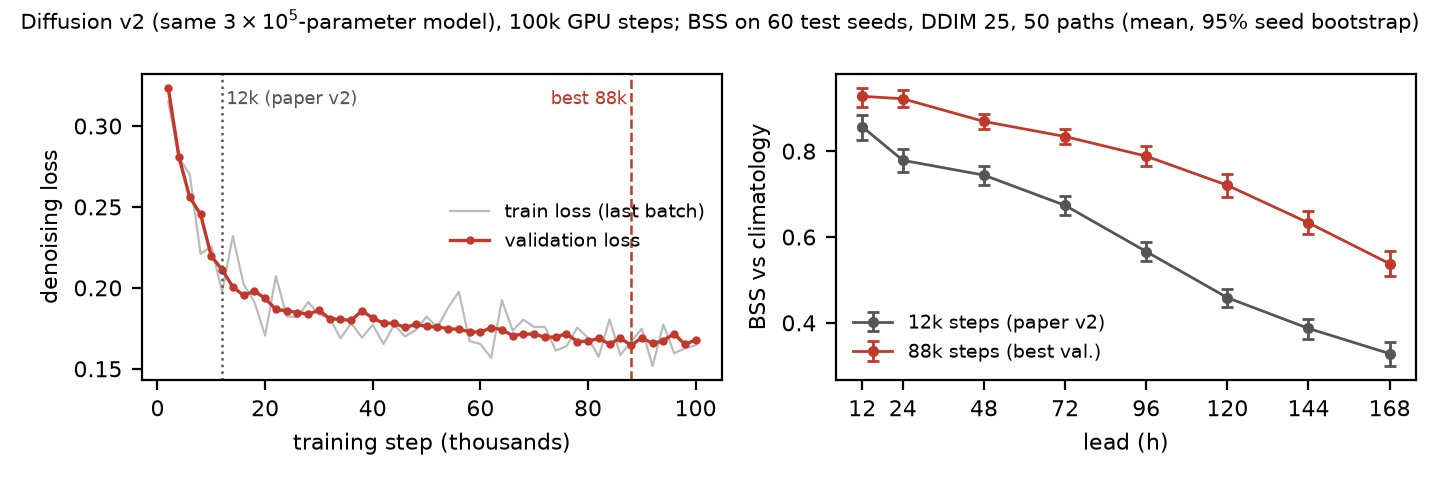
\includegraphics[width=0.9\linewidth]{figures/e1_learning_curve}
\caption{Learning curve of the $3\times10^5$-parameter diffusion model
(endurance, murky). Left: denoising loss on the validation split every 2{,}000
steps over 100{,}000 GPU steps; dotted line = the 12k-step ablation model, dashed line = best validation checkpoint. Right: Brier skill score
against climatology by lead on test seeds 220000--220059 (DDIM 25, 50 paths; mean and 95\%
seed-bootstrap interval) for the 12k-step model and the best checkpoint.}
\label{fig:lc}
\end{figure}

\paragraph*{Exile confounds survival time}
The ultimatum and furnace explosions bound the value of foresight measured in
days; we kept them, as in the shipped game, and measured per storm reached.
Per-storm metrics have their own selection effect (better colonies reach more
and later storms with more people), which pairing on identical storms and
normalising per 100 colonists only partly removes.

\paragraph*{Scope} The forecasting evaluation uses one dynamical system and a
handful of observation models; the game's daily temperature script makes part
of the cold clock-predictable. RL results come from one game and one
difficulty with three training runs per rung; training variance in colony
management is larger than the value of the storm date, so three runs bound the
ladder's ordering but not the size of its gaps, and they cannot order 3b and
3a$^{\prime}$. Table~\ref{tab:compute} lists the compute: CPU work ran on one
shared 15-core Apple M5 Pro, GPU work and the 3b/3a$^{\prime}$ PPO runs on one
laptop with an 8\,GB RTX 4060.

\begin{table}[t]
\centering
\caption{Compute (wall-clock). CPU: shared 15-core Apple M5 Pro unless
marked; GPU and ``laptop'': one laptop with an RTX 4060.}
\label{tab:compute}
\footnotesize
\setlength{\tabcolsep}{3pt}
\begin{tabular}{@{}p{0.64\columnwidth}r@{}}
\toprule
Step & Cost \\
\midrule
Weather data, 500 seeds $\times$ 120 days / PF oracle, per seed & 0.15\,s / 6\,s \\
GRU training, 16k steps (2 threads) & 53\,min \\
Diffusion v2, 12k steps (4 threads) & 2.6\,h \\
Diffusion v2, 100k steps & 2.3\,h GPU \\
Diffusion v3 selection, 9 runs $\times$ 100k steps & 36.6\,h GPU \\
Diffusion v3, 100k steps, per training seed & 5.1--5.3\,h GPU \\
Diffusion v2 sampling, 50 paths $\times$ 113 issues, per seed (4 threads) & 4.2\,min \\
200-seed evaluation, \pathsDiff{} paths, DDIM \ddimSteps: v2 & \gpuHoursTwo\,h GPU \\
\quad same, v3, per training seed & \gpuHoursThreeMin--\gpuHoursThreeMax\,h GPU \\
PPO, per run (200M steps, 8 envs) & 8.3--8.7\,h \\
\quad rung 3a (online GRU) & 13.5--14.9\,h \\
Daily forecast tables: diffusion v3 / GRU & \ebTableDiffHours\,h GPU / \ebTableGruMin\,min \\
PPO 3b / 3a$^{\prime}$, per run (6 concurrent, laptop CPU) & $\geq$\ebPpoHoursMin--\ebPpoHoursMax\,h \\
Wind-noise ablation: diffusion / PF + GRU & \wnGpuHours\,h GPU / \wnCpuHours\,h laptop \\
\bottomrule
\end{tabular}
\end{table}

%======================================================================
\section{Conclusion and Future Work}
%======================================================================
A survival game whose storms come from integer Lorenz-63 dynamics combines a
hazard that players must forecast with a near-exact predictive distribution
to grade forecasters against. A GRU landing-time classifier and two
conditional diffusion models are calibrated and close to one another on the
landing event, short of the oracle, and only the generative models produce
seven-day scenarios. For a PPO colony manager, the true storm date and a
history-integrating GRU forecast lower losses per storm relative to raw signs
in every run, raw signs give nothing reliable, and three runs cannot order the
diffusion and GRU forecasts as once-daily policy inputs. Next we will feed the
generated scenarios to a diffusion ``slow planner'' that drafts multi-day
camp plans for an in-game steward, a consumer of whole trajectories rather
than event probabilities.

\bibliographystyle{IEEEtran}
\bibliography{refs}

\end{document}
